
\chapter{Velocity balance} \label{ssn_balance_velocity}

\index{Balance equations!Velocity}
Due to the complexity of solving the higher-order Stokes models of Chapter \cref{ssn_momentum_and_mass_balance}, it is desirable to be able to run CPU-time-inexpensive computations over continent-scale regions.
One way to calculate a less-expensive momentum property is by solving the \emph{balance velocity}; the vertically-averaged velocity
\begin{align}
  \label{balance_velocity}
  \bar{\rankone{u}} = \frac{1}{H} \int_z \rankone{u} \d{z},
\end{align}
with components $\bar{\rankone{u}} = [\bar{u}\ \bar{v}\ \bar{w}]\T$.  

First, assume that a given volume of ice with density $\rho$ within an arbitrary domain $\Omega \in \R^3$ with boundary $\Gamma$ remains constant.
Applying Reynolds tranport \cref{constant_volume_reynolds} to the total time derivative term and inserting $\phi = \rho$, $\rankone{j} = \rho \rankone{u}$, and $f=0$ into continutity equation \cref{integral_continuity_equation} results in 
\begin{align}
  \label{general_mass_balance}
  \totder{}{t} \int_{\Omega} \rho \d{\Omega} = \int_{\Omega} \parder{\rho}{t} \d{\Omega} = - \int_{\Gamma} \rho \rankone{u} \cdot \rankone{n} \d{\Gamma}.
\end{align}
In the context of ice-sheets, there is a flux of ice across the upper surface $\Gamma_S$ by either accumulation or ablation $\dot{a}$, and a flux of ice lost across the basal surface $\Gamma_B$ by melting $F_b$.
Hence
\begin{align}
  \label{surface_mass_loss}
  \left( \rankone{w}_S - \rankone{u} \right) \cdot \rankone{n} |_{\Gamma_S} &= \dot{a} &&\text{ on } \Gamma_A  \\
  \label{basal_mass_loss}
  \left( \rankone{u} - \rankone{w}_B \right) \cdot \rankone{n} |_{\Gamma_B} &= F_b &&\text{ on } \Gamma_B ,
\end{align}
where $\rankone{w}_B$ and $\rankone{w}_S$ is the velocity of the free surfaces $F_S(\rankone{x},t) = z - S(x,y,t)$ and $F_B(\rankone{x},t) = B(x,y,t) - z$ at the coordinate $\rankone{x} = [x\ y\ z]\T$, respectively \citep{greve_1997}.  Therefore, the boundary integral of general mass balance relation \cref{general_mass_balance} may be decomposed into
\begin{align*}
  \int_{\Gamma} \rho \rankone{u} \cdot \rankone{n} \d{\Gamma} = &+ \int_{\Gamma_B} \rho \left( \rankone{w}_B \cdot \rankone{n} + F_b \right) \d{\Gamma_B} \\
  &+ \int_{\Gamma_S} \rho \left( \rankone{w}_S \cdot \rankone{n} - \dot{a} \right) \d{\Gamma_S} \\
  &+ \int_{\Gamma_L} \rho \rankone{u} \cdot \rankone{n} \d{\Gamma_L} 
\end{align*}
where $\Gamma_B$ is the basal surface, $\Gamma_S$ is the upper surface, and $\Gamma_L$ is the lateral surface of the volume.

Next, if the rate of change of the free surface $F_S(\rankone{x},t)$ and $F_B(\rankone{x},t)$ is unchanging, the Eulerian coordinate system demands that
\begin{align}
  \label{kinematic_surface}
  \totder{F_S}{t} &= \parder{F_S}{t} + \rankone{w}_S \cdot \nabla F_S = 0 \\
  \label{kinematic_bed}
  \totder{F_B}{t} &= \parder{F_B}{t} + \rankone{w}_B \cdot \nabla F_B = 0.
\end{align}
Using the outward-pointing normal vector definition on the surface and bed
\begin{align}
  \label{normal_vector}
  \rankone{n} |_{\Gamma_S} = \frac{\nabla F_S}{\Vert \nabla F_S \Vert}, \hspace{10mm}
  \rankone{n} |_{\Gamma_B} = \frac{\nabla F_B}{\Vert \nabla F_B \Vert},
\end{align}
and relations \cref{surface_mass_loss,basal_mass_loss},
\begin{align*}
  \rankone{w}_S \cdot \nabla F_S &= \Vert \nabla F_S \Vert \left( \dot{a} + \rankone{u} \cdot \frac{\nabla F_S}{\Vert \nabla F_S \Vert} \right) \\
  \rankone{w}_B \cdot \nabla F_B &= \Vert \nabla F_B \Vert \left( - F_b + \rankone{u} \cdot \frac{\nabla F_B}{\Vert \nabla F_B \Vert} \right),
\end{align*}
which used in \cref{kinematic_surface,kinematic_bed} results in  
\begin{align*}
  \parder{F_S}{t} + \rankone{u} \cdot \nabla F_S &= - \Vert \nabla F_S \Vert \dot{a} \\
  \parder{F_B}{t} + \rankone{u} \cdot \nabla F_B &= \Vert \nabla F_B \Vert F_b.
\end{align*}
Evaluating the derivatives above,
\begin{align*}
  \rankone{u} \cdot \nabla F_S &= \rankone{u} \cdot \left( \hat{\rankone{k}} - \nabla S \right) = - \Vert \hat{\rankone{k}} - \nabla S \Vert \dot{a} + \parder{S}{t} \\
  \rankone{u} \cdot \nabla F_B &= \rankone{u} \cdot \left( \nabla B - \hat{\rankone{k}} \right) = \Vert \nabla B - \hat{\rankone{k}} \Vert F_b - \parder{B}{t},
\end{align*}
and with the use of $\hat{\rankone{k}} \cdot \rankone{u}(\rankone{x},t) = w(\rankone{x},t)$, 
\begin{align}
  \label{u_dot_gradS}
  \rankone{u} |_{\Gamma_S} \cdot \nabla S &= w(S) + \Vert \hat{\rankone{k}} - \nabla S \Vert \dot{a} - \parder{S}{t} \\
  \label{u_dot_gradB}
  \rankone{u} |_{\Gamma_B} \cdot \nabla B &= w(B) + \Vert \nabla B - \hat{\rankone{k}} \Vert F_b - \parder{B}{t}.
\end{align}

Next, employing \index{Divergence theorem!Regarding velocity balance} divergence \cref{divergence_theorem} to the boundary integral in general mass balance \cref{general_mass_balance} results in
\begin{align*}
  \totder{}{t} \int_{\Omega} \rho \d{\Omega} + \int_{\Omega} \rho \nabla \cdot \rankone{u} \d{\Omega} = \int_{\Omega} \left( \parder{\rho}{t} + \rho \nabla \cdot \rankone{u} \right) \d{\Omega} = 0,
\end{align*}
and thus
\begin{align*}
  \parder{\rho}{t} + \rho \nabla \cdot \rankone{u} = 0.
\end{align*}
Due to the fact that ice is incompressible, $\partial_t \rho = 0$ and conservation of mass relation \cref{cons_mass}, $\nabla \cdot \rankone{u} = 0$, has been derived.
Integrating this expression vertically, applying \index{Leibniz's rule} Leibniz's rule \cref{leibniz_rule} \index{Leibniz's rule!Velocity balance}, and using the first fundamental theorem of calculus (\cf. \cref{first_fundamental_theorem_of_calculus}),
\begin{align}
  \label{integrated_cons_mass}
  \nabla \cdot \left( \int_B^S \rankone{u} \d{z} \right) + \rankone{u} |_{\Gamma_B} \cdot \nabla B - \rankone{u} |_{\Gamma_S} \cdot \nabla S + w(S) - w(B) = 0,
\end{align}
which using balance-velocity definition \cref{balance_velocity} and inserting \cref{u_dot_gradS,u_dot_gradB} produces
\begin{align*}
  \nabla \cdot \big( H \bar{\rankone{u}} \big) = &+ \rankone{u} |_{\Gamma_S} \cdot \nabla S - \rankone{u} |_{\Gamma_B} \cdot \nabla B - w(S) + w(B) \\
  =&+ \left( w(S) + \Vert \hat{\rankone{k}} - \nabla S \Vert \dot{a} - \parder{S}{t}\right) - w(S) \\
  &- \left( w(B) + \Vert \nabla B - \hat{\rankone{k}} \Vert F_b - \parder{B}{t} \right) + w(B) \\
  =& \Vert \hat{\rankone{k}} - \nabla S \Vert \dot{a} - \Vert \nabla B - \hat{\rankone{k}} \Vert F_b - \parder{H}{t}
\end{align*}
where in the last step, ice thickness definition $H(x,y) = S(x,y) - B(x,y)$ has been used.

Finally, we can state the \emph{balance velocity equation}
\begin{align}
  \label{balance_velocity_equation_one}
  \nabla \cdot \big( H \bar{\rankone{u}} \big) = f,
\end{align}
with forcing term
\begin{align}
  \label{balance_velocity_equation_f}
  f = \Vert \hat{\rankone{k}} - \nabla S \Vert \dot{a} - \Vert \nabla B - \hat{\rankone{k}} \Vert F_b - \parder{H}{t}.
\end{align}

Note that the rate of change of the thickness $\partial_t H$ and the surface accumulation/ablation rate $\dot{a}$ may be estimated from observations and the mass loss due to basal water melting $F_b$ can be attained by the methods of Chapter \cref{ssn_internal_energy_balance}.

\section{The direction of flowing ice}

Balance velocity $\bar{\rankone{u}}$ may be decomposed into a direction $\hat{\rankone{u}}$ and magnitude $\bar{u}$ \citep{brinkerhoff_2015} such that
\begin{align}
  \label{balance_velocity_dir_and_mag}
  \bar{\rankone{u}} = \bar{u} \rankone{\hat{u}},
\end{align}
with unit vector $\hat{\rankone{u}} = [\hat{u}\ \hat{v}\ \hat{w}]\T$.  From balance equation \cref{balance_velocity_equation_one},
\begin{align}
  \label{balance_velocity_equation}
  \nabla \cdot \big( H \bar{u} \rankone{\hat{u}} \big) &= f,
\end{align}
which can be expanded with terms $H$ and $\hat{u}$ grouped together,
\begin{align*}
  \bar{u} H \nabla \cdot \rankone{\hat{u}} + \nabla \big( \bar{u} H \big) \cdot \rankone{\hat{u}} &= f \\
  \bar{u} H \nabla \cdot \rankone{\hat{u}} + \big( H \nabla \bar{u} + \bar{u} \nabla H \big) \cdot \rankone{\hat{u}} &= f.
\end{align*}
After a little rearranging, this produces
\begin{align}
  H \hat{\rankone{u}} \cdot \nabla \bar{u} + \big( H \nabla \cdot \rankone{\hat{u}} + \nabla H \cdot \rankone{\hat{u}} \big) \bar{u} &= f \notag \\
  \label{balance_velocity_equation_expanded}
  H \hat{\rankone{u}} \cdot \nabla \bar{u} + \nabla \cdot \big( H \rankone{\hat{u}} \big) \bar{u} &= f.
\end{align}

Next, because this system includes one equation and three unknowns, two are eliminated by \emph{prescribing} the direction of flow.  In the absence of surface velocity data, one choice for this direction is down the gradient of \index{Driving stress} \emph{driving stress} $\rankone{\tau_d} = [\tau_x\ \tau_y\ 0]\T$, derived by integrating vertically the forcing term of first-order momentum balance \cref{bp_cons_momentum}:
\begin{align}
  \label{driving_stress}
  \rankone{\tau_d} = \int_B^S \rho g \nabla S \d{z} = \rho g H \nabla S.
\end{align}

Upon closer inspection of balance velocity relation \cref{balance_velocity_equation_one}, and using the fact that the partial derivative of the vertically integrated velocity with respect to $z$ is zero,
\begin{align*}
  \nabla \cdot \big( H \bar{\rankone{u}} \big) &= \parder{}{x} \left( \int_B^S \rankone{u} \d{z} \right)
     + \parder{}{y} \left( \int_B^S \rankone{u} \d{z} \right).
\end{align*}
Hence only the two horizontal components $\hat{u}$ and $\hat{v}$ of balance velocity \cref{balance_velocity} remain, and the domain is reduced to $\Omega \in \R^2$.  Additionally, because only the \emph{direction} of ice flow is imposed, the direction $\nabla S$ may be used in place of full driving stress \cref{driving_stress}.

Let the direction of imposed flow be defined as
\begin{align}
  \label{balance_velocity_direction}
  \hat{\rankone{u}} = \frac{\rankone{d}}{\Vert \rankone{d} \Vert}, \hspace{10mm} 
  \rankone{d} = \begin{bmatrix}
                 d_x \\
                 d_y \\
               \end{bmatrix}.
\end{align}
Due to the fact that the solution to balance-velocity Equation \cref{balance_velocity_equation,balance_velocity_equation_f} will be highly sensitive to variations in the data used to define \cref{balance_velocity_direction}, an additional term is added to flow-direction \cref{balance_velocity_direction} in such a way that direction is decomposed into data $\rankone{d}^{\text{data}}$ and Laplace-blurring $\rankone{d}^s$ terms \citep{brinkerhoff_2015}
\begin{align*}
  \rankone{d} &= \rankone{d}^{\text{data}} + \rankone{d}^s, \hspace{5mm} \rankone{d}^s = \big( \kappa H \big)^2 \nabla \cdot \big( \nabla \rankone{d} \big),
\end{align*}
where the constant $\kappa$ adjusts the amount of smoothing proportional to the ice thickness $H$.  The expansion of this linear system is
\begin{align*}
  \begin{bmatrix}
    d_x \\
    d_y
  \end{bmatrix} - \big( \kappa H \big)^2
  \begin{bmatrix}
    \parder[2]{d_x}{x} + \parder[2]{d_x}{y} \\ 
    \parder[2]{d_y}{x} + \parder[2]{d_y}{y}
  \end{bmatrix} &=
  \begin{bmatrix}
     d_x^{\text{data}} \\
     d_y^{\text{data}}
  \end{bmatrix},
\end{align*}
thus illuminating two equations for the unknowns $d_x$ and $d_y$,
\begin{align}
  \label{smoothed_driving_stress_x}
  d_x - \big( \kappa H \big)^2 \left( \parder[2]{d_x^s}{x} + \parder[2]{d_x^s}{y} \right) &= d_x^{\text{data}} \\
  \label{smoothed_driving_stress_y}
  d_y - \big( \kappa H \big)^2 \left( \parder[2]{d_y^s}{x} + \parder[2]{d_y^s}{y} \right) &= d_y^{\text{data}}.
\end{align}

\subsection{Variational forms}

The variational problem associated with smoothed driving stress Equations \cref{smoothed_driving_stress_x,smoothed_driving_stress_y} reads: find $d_x \in \ltwospace$ (see $L^2$ space \cref{l2_space}) such that
\begin{align*}
  \int_{\Omega} d_x \phi \d{\Omega} - \int_{\Omega} \big( \kappa H \big)^2 \left( \parder[2]{d_x}{x} + \parder[2]{d_x}{y} \right) \phi \d{\Omega} &= \int_{\Omega} d_x^{\text{data}} \phi \d{\Omega} \\
  \int_{\Omega} d_x \phi \d{\Omega} + \int_{\Omega} \big( \kappa H \big)^2 \big( \nabla d_x \big)_h \cdot \big( \nabla \phi \big)_h \d{\Omega} &\\
  - \int_{\Gamma} \phi \big( \kappa H \big)^2 \big( \nabla d_x \big)_h \cdot \rankone{n}_h \d{\Gamma} &= \int_{\Omega} d_x^{\text{data}} \phi \d{\Omega}
\end{align*}
for all $\phi \in \testspace$ (see test space \cref{test_space}); and $d_y \in \ltwospace$ such that
\begin{align*}
  \int_{\Omega} d_y \psi \d{\Omega} - \int_{\Omega} \big( \kappa H \big)^2 \left( \parder[2]{d_y}{x} + \parder[2]{d_y}{y} \right) \psi \d{\Omega} &= \int_{\Omega} d_y^{\text{data}} \psi \d{\Omega} \\
  \int_{\Omega} d_y \psi \d{\Omega} + \int_{\Omega} \big( \kappa H \big)^2 \big( \nabla d_y \big)_h \cdot \big( \nabla \psi \big)_h \d{\Omega} &\\
  - \int_{\Gamma} \psi \big( \kappa H \big)^2 \big( \nabla d_y \big)_h \cdot \rankone{n}_h \d{\Gamma} &= \int_{\Omega} d_y^{\text{data}} \psi \d{\Omega}
\end{align*}
for all $\psi \in \testspace$.  Horizontal vector components are denoted $\rankone{v}_h = [v_x\ v_y]\T$.

\section{The magnitude of flowing ice}

On closer examination of velocity-balance relation \cref{balance_velocity_equation_expanded}, the equation is seen to be of the same form as the advection-reaction equation described in \cref{ssn_stabilized_methods},
\begin{align*}
  \rankone{a} \cdot \nabla u + s u = f,
\end{align*}
with unknown quantity $u = \bar{u}$, velocity $\rankone{a} = H \hat{\rankone{u}}$, and reaction coefficient $s = \nabla \cdot \big( H \rankone{\hat{u}} \big)$.  As previously discussed in \cref{ssn_stabilized_methods}, equations of this type suffer from numerical oscillations requiring the use of stabilization.  Therefore, defining the linear differential operator associated with problem \cref{balance_velocity_equation_expanded},
\begin{align}
  \label{bv_linear_operator}
  \Lu u &= H \hat{\rankone{u}} \cdot \nabla \bar{u} + \nabla \cdot \big( H \rankone{\hat{u}} \big) \bar{u},
\end{align}
the stabilized form is stated using general stabilized form \cref{generalized_form} with test function $\phi \in \testspace$ and intrinsic-time parameter \index{Intrinsic-time parameter!Balance velocity} $\tau_{\text{BV}}$,
\begin{align}
  \label{bv_generalized_form}
  (\phi, \Lu \bar{u}) + (\mathbb{L} \phi, \tau_{\text{BV}}(\Lu\bar{u} - f)) &= (\phi, f),
\end{align}
where operator $\mathbb{L}$ is a differential operator typically chosen from
\begin{align}
  \label{bv_gls_operator}
  \mathbb{L} &= + \Lu && \text{Galerkin/least-squares (GLS)} \\
  \label{bv_supg_operator}
  \mathbb{L} &= + \Lu_{\text{adv}} && \text{SUPG} \\
  \label{bv_ssm_operator}
  \mathbb{L} &= - \Lu^* && \text{subgrid-scale model (SSM)}
\end{align}
with $\Lu_{\text{adv}} = H\hat{\rankone{u}} \cdot \nabla \bar{u}$, the advective part of the operator $\Lu$.

An appropriate stabilization parameter for this problem is given by \cref{tau_adr}, as derived by \citet{codina_1992}.  After making the appropriate substitutions to ADR parameter \cref{tau_adr}, the intrinsic-time parameter is
\begin{align}
  \label{tau_bv}
  \tau_{\text{BV}} = \frac{1}{\frac{2 H}{h} + \nabla \cdot \big( H \hat{\rankone{u}} \big)},
\end{align}
with cell diameter $h$.  Here, the fact that $\Vert \hat{\rankone{u}} \Vert = 1$ and that there is no diffusion present has been used.

\subsection{Variational form}

Using intrinsic-time parameter \cref{tau_bv} and operator \cref{bv_linear_operator}, the variational problem associated with \cref{balance_velocity_equation,balance_velocity_equation_f} reads: find $\bar{u} \in \ltwospace$ such that
\begin{align}
  \label{balance_velocity_weak_problem}
  \mathscr{B}(\phi, \bar{u}) = \ell(\phi),
\end{align}
where
\begin{align*}
  \mathscr{B}(\phi, \bar{u} &= (\phi, \Lu \bar{u}) + (\mathbb{L} \phi, \tau_{\text{BV}}(\Lu\bar{u})) \\
  \ell(\phi) &= (\phi, f) + (\mathbb{L} \phi, \tau_{\text{BV}}f),
\end{align*}
for all $\phi \in \trialspace$ and $\mathbb{L}$ given by one of \cref{bv_gls_operator}, \cref{bv_supg_operator}, or \cref{bv_ssm_operator}.

The implementation of this problem by \CSLVR is shown in \cref{cslvr_balance_velocity}.

\pythonexternal[label=cslvr_balance_velocity, caption={\CSLVR implementation of the \texttt{BalanceVelocity} class.}]{cslvr_src/balancevelocity.py}

\section{Continent-wide simulations} \label{ssn_balance_velocity_simulations}

\index{Linear differential equations!2D}
Solutions to balance-velocity variational problem \cref{balance_velocity_weak_problem} were obtained over the entire continents of Antarctica and Greenland for each of stabilization schemes \cref{bv_gls_operator,bv_supg_operator,bv_ssm_operator}.
In order to complete these simulations, some assumptions had to be made regarding forcing term \cref{balance_velocity_equation_f}: we assume that the ice sheet thickness is in equilibrium, and hence $\partial_t H = 0$ and do not prescribe any basal melting such that $F_b = 0$.

To create the finite-element mesh, we incorporated the dynamic version of GMSH \citep{geuzaine_2009} into \CSLVR.  This software allows us to generate finite-element meshes with cell diameters set by any function we wish.  Following the work of \citet{brinkerhoff_2015}, we generated meshes for each ice-sheet with cell diameter $h$ given by 
$$h = mH$$
for some constant $m$.

Finally, simulations were run using flow directions $\rankone{d}^{\text{data}}$ both in the down-surface-gradient direction \cref{balance_velocity_direction} and in the direction of surface observations $\rankone{u}_{ob}$ (\cref{greenland_u_ob_image,antarctica_u_ob_image}).
Due to the fact that the surface gradient is nearly zero over the floating shelves of Antarctica, the flow direction resulting from the surface gradient is not well defined.
To investigate this problem, we applied the direction of flow to be in the direction of surface velocity observations $\rankone{u}_{ob} = [u_{ob}\ v_{ob}]\T$ in these areas, with improved results (\cref{antarctica_bv_image_U_ob_S}).
For comparison purposes, we then ran a simulation over Antarctica imposing the direction of flow entirely in the direction of observations $\rankone{u}_{ob}$, and noticed that the results obtained without smoothing contained high error in regions without velocity observations (\cref{antarctica_bv_image_d_U_ob}).
To remedy this, we ran one final test over Antarctica with direction of flow imposed in the direction of velocity observations $\rankone{u}_{ob}$ where observations are present and down the surface gradient $\nabla S$ where they are not (\cref{antarctica_bv_image_d_gS_m_U}).

Results indicate that the vertically averaged flow field $\bar{u}$ roughly reproduces the general pattern of recorded surface velocities over both Greenland (\cref{greenland_bv_image,greenland_bv_image_d_U_ob}) and Antarctica (\cref{antarctica_bv_image,antarctica_bv_image_d_U_ob}).
The difference between the vertically-averaged velocity and the recorded surface speed provides some insight into the variation of velocity with depth (\cref{greenland_bv_image_misfit,greenland_bv_image_d_U_ob_misfit,antarctica_bv_image_misfit,antarctica_bv_image_U_ob_S_misfit,antarctica_bv_image_U_ob_misfit,antarctica_bv_image_gS_m_U_misfit}).
That is, in regions where the misfit is high, we expect significant differences between the surface and the basal velocity.
However, due to the fact that the data---including topography, accumulation, $\partial_t H$ and $F_b$---contain a high degree of uncertainty, we expect that with better data the sporadic variance structure evident here will be diminished.

Defining the direction of flow in the direction of velocity observations over the shelves of Antarctica is an improvement over the down-surface-gradient direction (compare \cref{antarctica_bv_image,antarctica_bv_image_U_ob_S}).
However, there appear to remain substantial differences between these two velocities in these regions (\cref{antarctica_bv_image_U_ob_S_misfit}).
This may be due to substantial basal melt or freeze-on under the shelves, implying in this case that our specification of $F_b = 0$ is entirely inappropriate.  Additionally, the balance velocity changes from under-estimation to over-estimation of the surface velocity over the fastest-moving parts of interior regions when a meaningful direction of flow is imposed over floating-ice regions (compare \cref{antarctica_bv_image_misfit,antarctica_bv_image_U_ob_S_misfit}).
This illuminates the fact that the balance velocity of the floating-ice shelves has at least some affect on the velocity deep within the interior.

Filling in the gaps of missing velocity data $\rankone{u}_{ob}$ with $-\nabla S$ appeared to have the most effect on results derived without smoothing (\cref{antarctica_bv_image_d_gS_m_U,antarctica_bv_image_gS_m_U_misfit}).

Finally, the solutions attained with the stabilization schemes \cref{bv_gls_operator,bv_supg_operator,bv_ssm_operator} varied most with lower values of smoothing radius $\kappa$.
At the lowest $\kappa$ values, the GLS model appears to on-average under estimate the velocity, while the SSM model seems to on-average over estimate.
Remarkably, all calculations over estimate the velocity of Southwest Greenland (\cref{greenland_bv_image_misfit,greenland_bv_image_d_U_ob_misfit}) and match the deep-interior velocity observations of Antarctica relatively well (\cref{antarctica_bv_image_misfit,antarctica_bv_image_U_ob_S_misfit,antarctica_bv_image_U_ob_misfit,antarctica_bv_image_gS_m_U_misfit}). 

\subsection{Greenland}

The Greenland simulations used topography $S$ and $B$ given by \citet{bamber_2013}, and an accumulation/ablation function $\dot{a}$ provided by \citet{annoortvanvanderveen_2001,burgess_2010}.

The \CSLVR scripts used to generate the mesh, data, and perform the simulation are shown in \cref{cslvr_greenland_gen_mesh}, \cref{cslvr_greenland_gen_data}, and \cref{cslvr_greenland_bv}, respectively. 

\begin{table}[H]
\centering
\caption[Greenland balance-velocity variables]{Greenland $\bar{u}$ simulation variables.}
\label{greenland_balance_velocity_values}
\begin{tabular}{llll}
\hline
\textbf{Variable} & \textbf{Value} & \textbf{Units} & \textbf{Description} \\
\hline
$\partial_t H$ & $0$     & m a\sups{-1}  & $H$ obs.~rate of change \\
$F_b$          & $0$     & m a\sups{-1}  & basal water discharge \\
$m$            & $5$     & --            & mesh refinement \\
$N_e$          & $92855$ & --            & number of cells \\
$N_n$          & $49064$ & --            & number of vertices \\
\hline
\end{tabular}
\end{table}

\pythonexternal[label=cslvr_greenland_gen_mesh, caption={\CSLVR script used to generate the 2D mesh for Greenland.}]{scripts/balance_velocity/greenland/gen_mesh.py}

\pythonexternal[label=cslvr_greenland_gen_data, caption={\CSLVR script used to generate the data used by the Greenland balance velocity calculation of \cref{cslvr_greenland_bv}.}]{scripts/balance_velocity/greenland/gen_data.py}

\pythonexternal[label=cslvr_greenland_bv, caption={\CSLVR script used to calculate the balance velocity for Greenland.}]{scripts/balance_velocity/greenland/balance_velocity.py}

\subsection{Antarctica}

The Antarctica simulations used topography $S$ and $B$ provided by \citet{fretwell_2013}, and an accumulation/ablation function $\dot{a}$ provided by \citet{arthern_2006,lebrocq_2010}.

The \CSLVR scripts used to generate the mesh, data, and perform the simulation are shown in \cref{cslvr_antarctica_gen_mesh,cslvr_antarctica_gen_data,cslvr_antarctica_bv}. 

\begin{table}[H]
\centering
\caption[Antarctica balance-velocity variables]{Antarctica $\bar{u}$ simulations variables.}
\label{antarctica_balance_velocity_values}
\begin{tabular}{llll}
\hline
\textbf{Variable} & \textbf{Value} & \textbf{Units} & \textbf{Description} \\
\hline
$\partial_t H$ & $0$       & m a\sups{-1}  & $H$ obs.~rate of change \\
$F_b$          & $0$       & m a\sups{-1}  & basal water discharge \\
$m$            & $10$      & --            & mesh refinement \\
$N_e$          & $162211$  & --            & number of cells \\
$N_n$          & $82894$   & --            & number of vertices \\
\hline
\end{tabular}
\end{table}

\pythonexternal[label=cslvr_antarctica_gen_mesh, caption={\CSLVR script used to generate the 2D mesh for Antarctica.}]{scripts/balance_velocity/antarctica/gen_mesh.py}

\pythonexternal[label=cslvr_antarctica_gen_data, caption={\CSLVR script used to generate the data used by the Antarctica balance velocity calculation of \cref{cslvr_antarctica_bv}.}]{scripts/balance_velocity/antarctica/gen_data.py}

\pythonexternal[label=cslvr_antarctica_bv, caption={\CSLVR script used to calculate the balance velocity for Antarctica.}]{scripts/balance_velocity/antarctica/balance_velocity.py}

%===============================================================================

\begin{figure*}
  \centering
    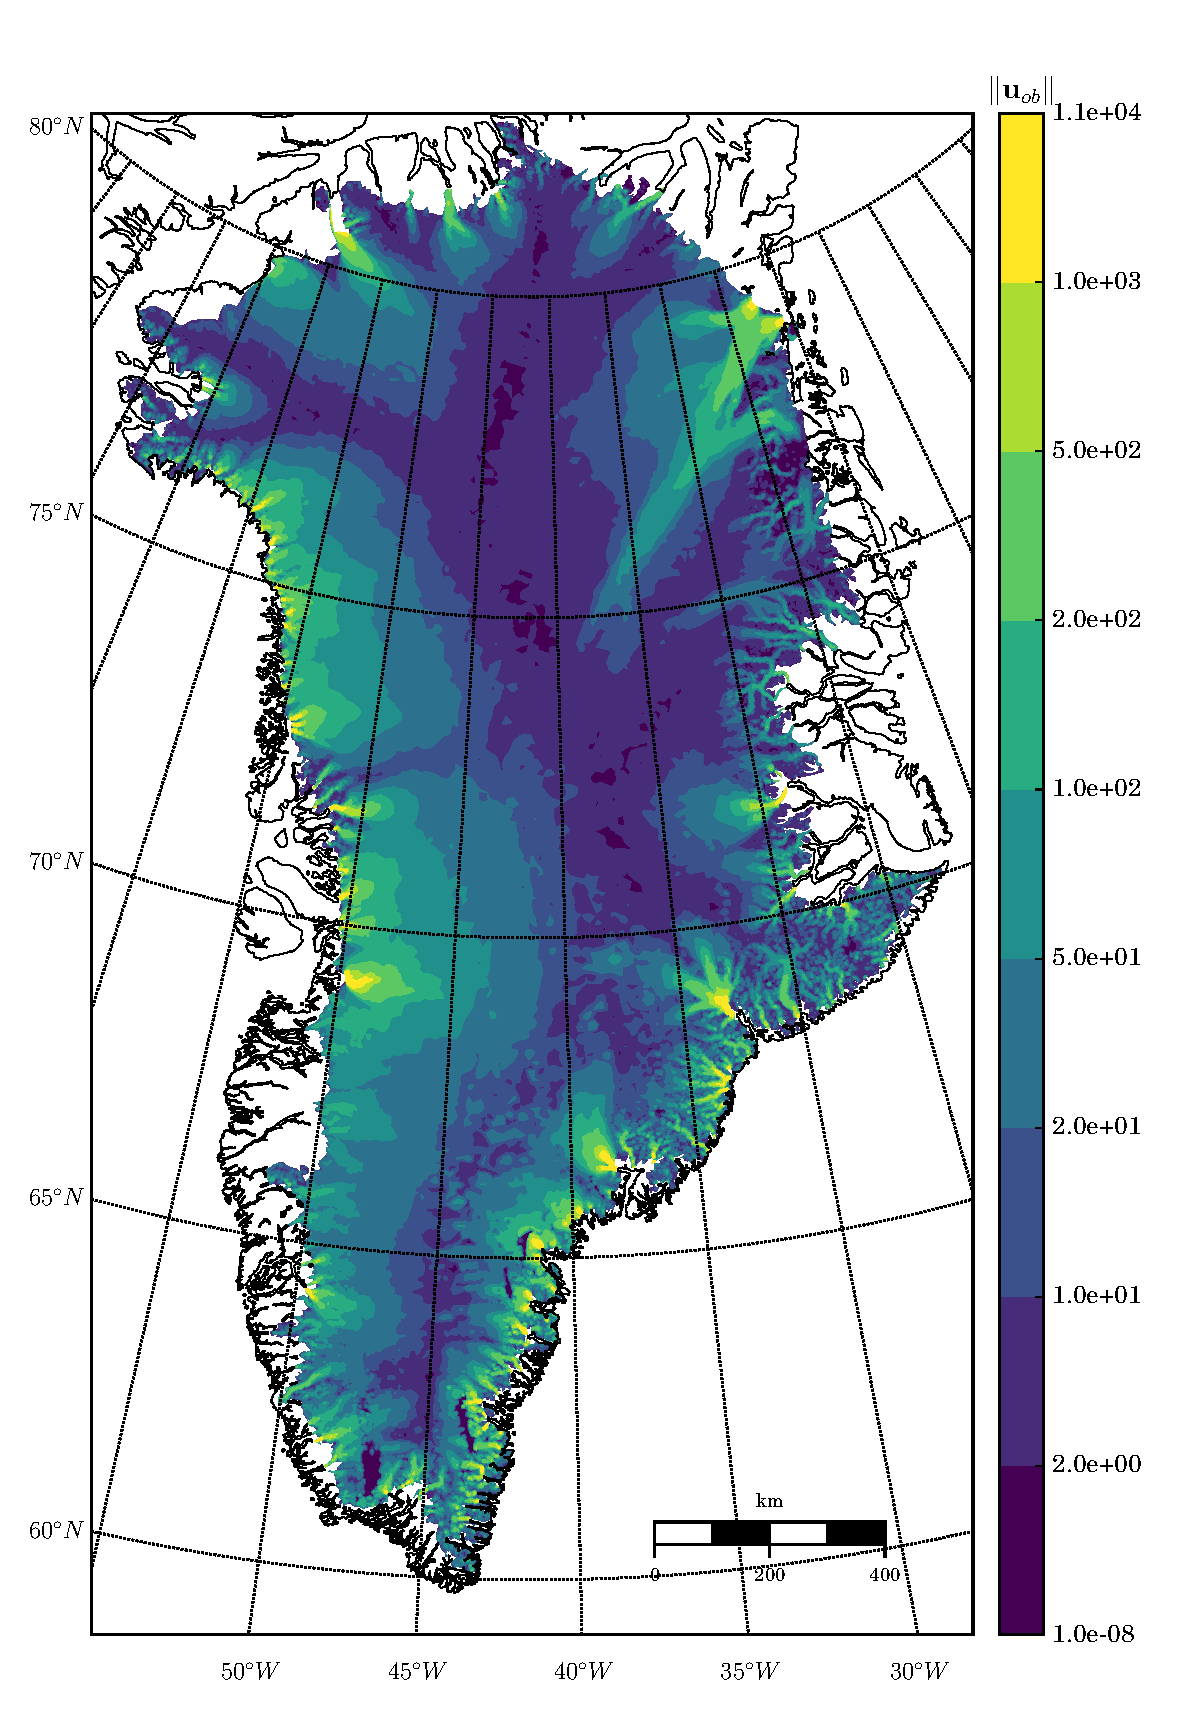
\includegraphics[width=0.8\linewidth]{images/balance_velocity/greenland/U_ob.pdf}
  \caption[Greenland surface-velocity magnitude]{Surface velocity magnitude of Greenland for the polar year 2008--2009 provided by \citet{rignot_2012}.}
  \label{greenland_u_ob_image}
\end{figure*}

%===============================================================================

\begin{figure*}
  
  \centering 

  \begin{subfigure}[b]{0.25\linewidth}
    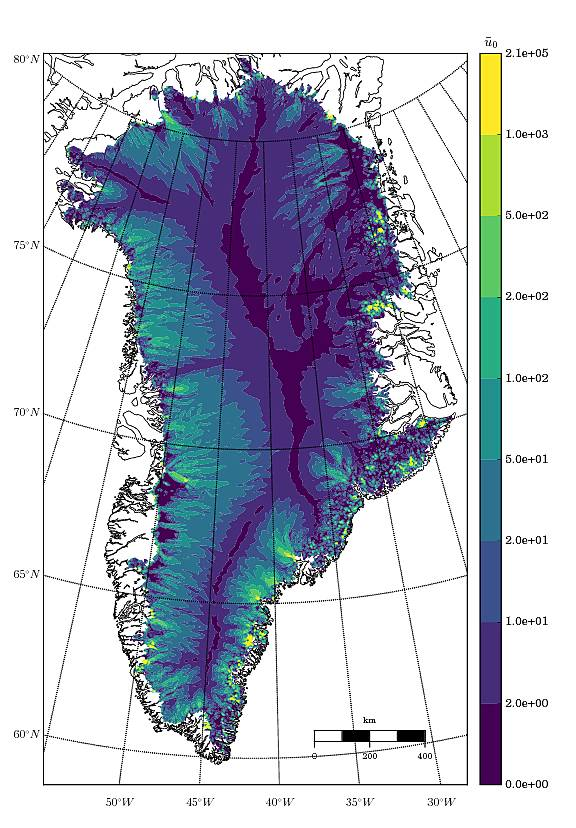
\includegraphics[width=\linewidth]{images/balance_velocity/greenland/Ubar_5H_kappa_0_GLS.jpg}
  \caption{$\kappa = 0$, GLS.}
  \label{greenland_bv_image_kappa_0_GLS}
  \end{subfigure}
  \begin{subfigure}[b]{0.25\linewidth}
    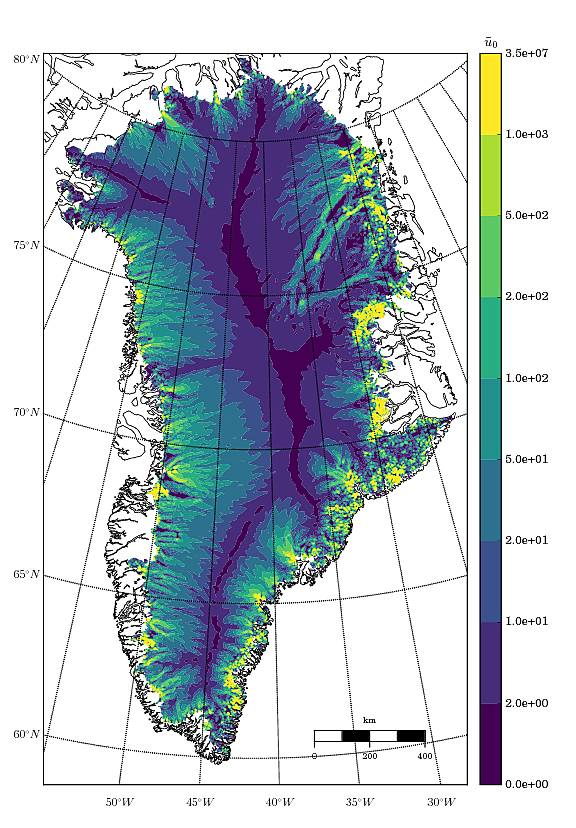
\includegraphics[width=\linewidth]{images/balance_velocity/greenland/Ubar_5H_kappa_0_SUPG.jpg}
  \caption{$\kappa = 0$, SUPG.}
  \label{greenland_bv_image_kappa_0_SUPG}
  \end{subfigure}
  \begin{subfigure}[b]{0.25\linewidth}
    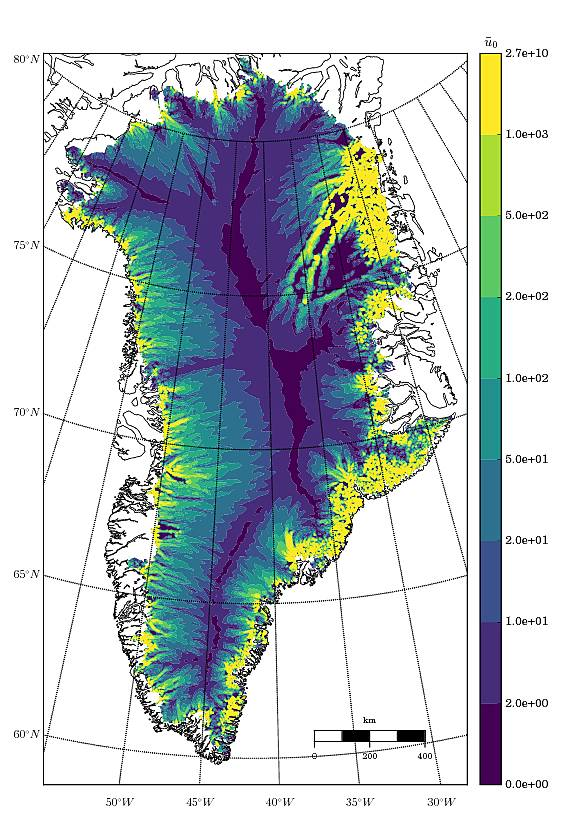
\includegraphics[width=\linewidth]{images/balance_velocity/greenland/Ubar_5H_kappa_0_SSM.jpg}
  \caption{$\kappa = 0$, SSM.}
  \label{greenland_bv_image_kappa_5_SSM}
  \end{subfigure}

  \begin{subfigure}[b]{0.25\linewidth}
    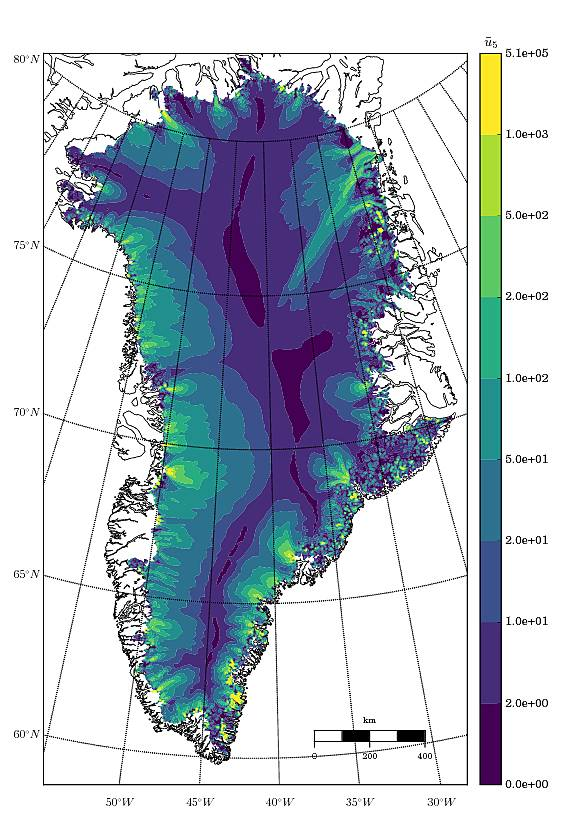
\includegraphics[width=\linewidth]{images/balance_velocity/greenland/Ubar_5H_kappa_5_GLS.jpg}
  \caption{$\kappa = 5$, GLS.}
  \label{greenland_bv_image_kappa_5_GLS}
  \end{subfigure}
  \begin{subfigure}[b]{0.25\linewidth}
    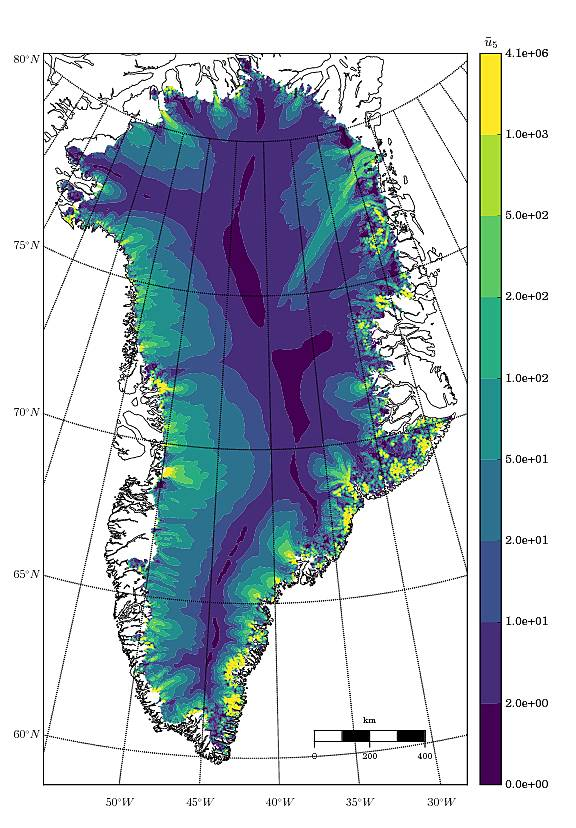
\includegraphics[width=\linewidth]{images/balance_velocity/greenland/Ubar_5H_kappa_5_SUPG.jpg}
  \caption{$\kappa = 5$, SUPG.}
  \label{greenland_bv_image_kappa_5_SUPG}
  \end{subfigure}
  \begin{subfigure}[b]{0.25\linewidth}
    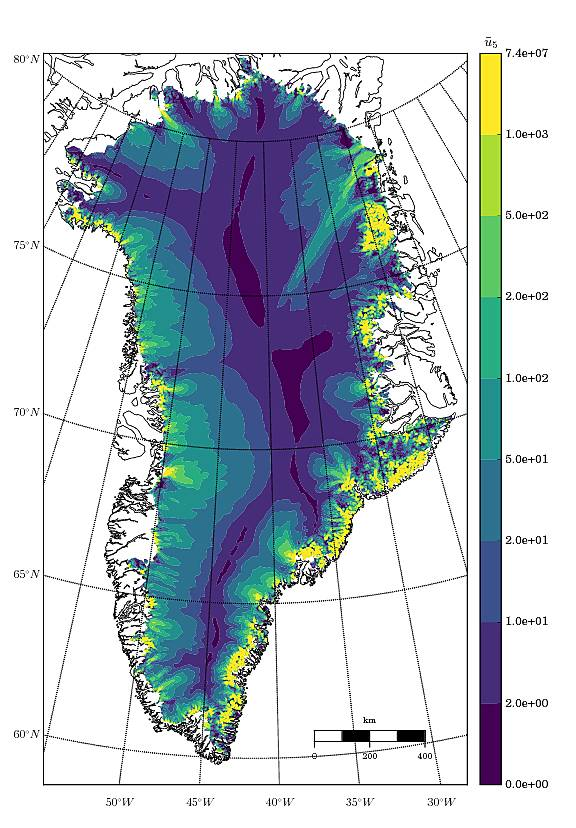
\includegraphics[width=\linewidth]{images/balance_velocity/greenland/Ubar_5H_kappa_5_SSM.jpg}
  \caption{$\kappa = 5$, SSM.}
  \label{greenland_bv_image_kappa_5_SSM}
  \end{subfigure}

  \begin{subfigure}[b]{0.25\linewidth}
    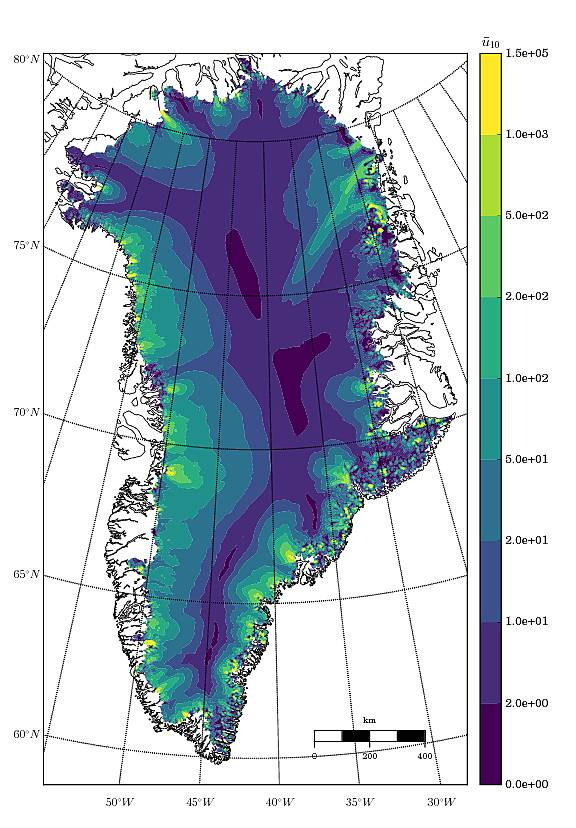
\includegraphics[width=\linewidth]{images/balance_velocity/greenland/Ubar_5H_kappa_10_GLS.jpg}
  \caption{$\kappa = 10$, GLS.}
  \label{greenland_bv_image_kappa_10_GLS}
  \end{subfigure}
  \begin{subfigure}[b]{0.25\linewidth}
    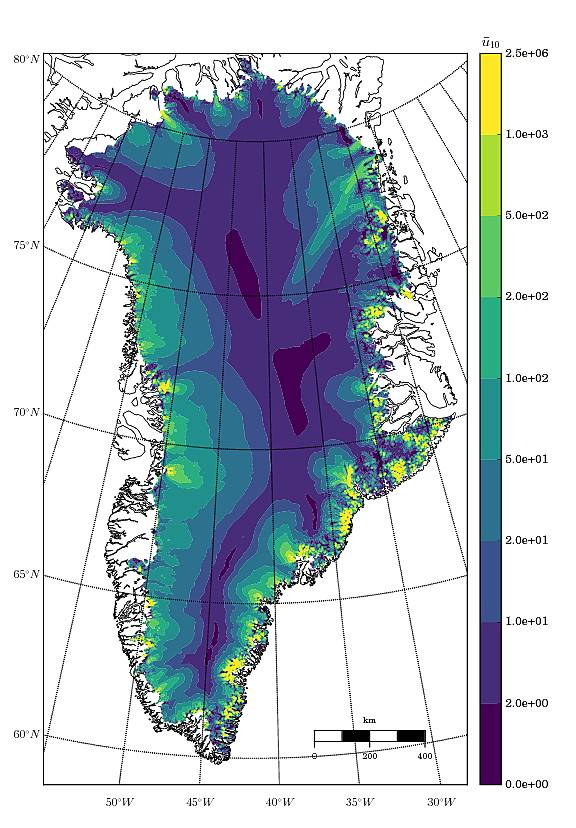
\includegraphics[width=\linewidth]{images/balance_velocity/greenland/Ubar_5H_kappa_10_SUPG.jpg}
  \caption{$\kappa = 10$, SUPG.}
  \label{greenland_bv_image_kappa_10_SUPG}
  \end{subfigure}
  \begin{subfigure}[b]{0.25\linewidth}
    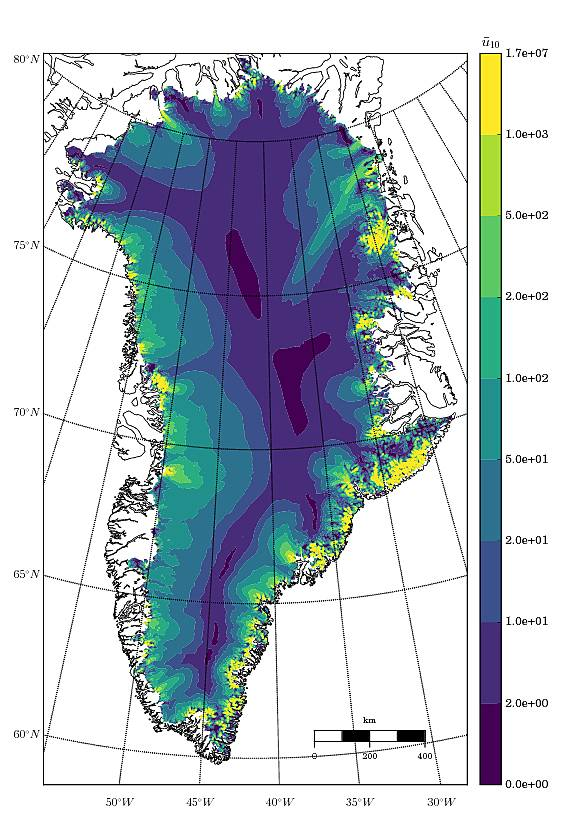
\includegraphics[width=\linewidth]{images/balance_velocity/greenland/Ubar_5H_kappa_10_SSM.jpg}
  \caption{$\kappa = 10$, SSM.}
  \label{greenland_bv_image_kappa_10_SSM}
  \end{subfigure}
 
  \caption[Greenland balance-velocity with $\mathbf{d}^{\text{data}} = -\nabla S$.]{Balance velocity $\bar{u}$ derived over Greenland with direction of flow imposed down the surface gradient $\nabla S$, where smoothing radius $\kappa$ varies as indicated.  The columns vary according to stabilization used; either Galerkin/least-squares (GLS) stabilization \cref{bv_gls_operator}, streamline-upwind/Petrov-Galerkin (SUPG) stabilization \cref{bv_supg_operator}, or subgrid-scale-model (SSM) stabilization \cref{bv_ssm_operator} in variational form \cref{balance_velocity_weak_problem}. \newline}

  \label{greenland_bv_image}

\end{figure*}

%===============================================================================

\begin{figure*}
  
  \centering 

  \begin{subfigure}[b]{0.25\linewidth}
    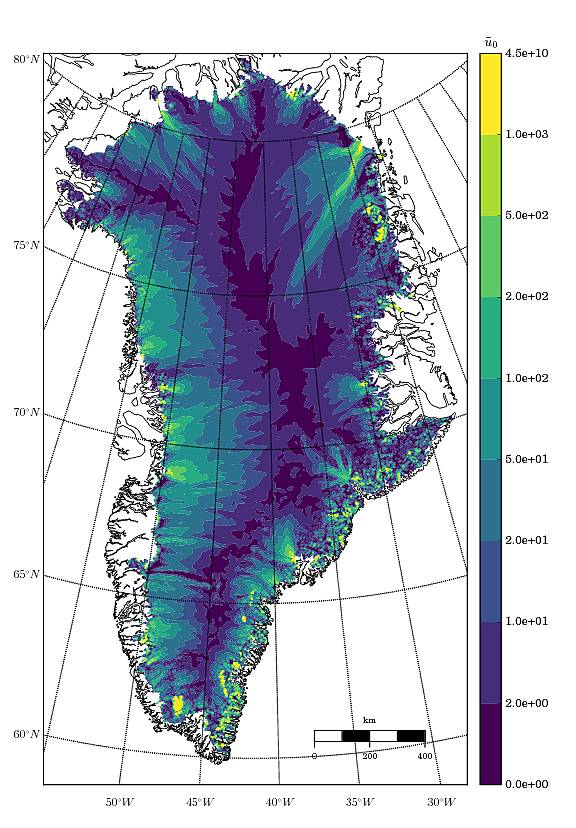
\includegraphics[width=\linewidth]{images/balance_velocity/greenland/d_U_ob/Ubar_5H_kappa_0_GLS.jpg}
  \caption{$\kappa = 0$, GLS.}
  \label{greenland_bv_image_d_U_ob_kappa_0_GLS}
  \end{subfigure}
  \begin{subfigure}[b]{0.25\linewidth}
    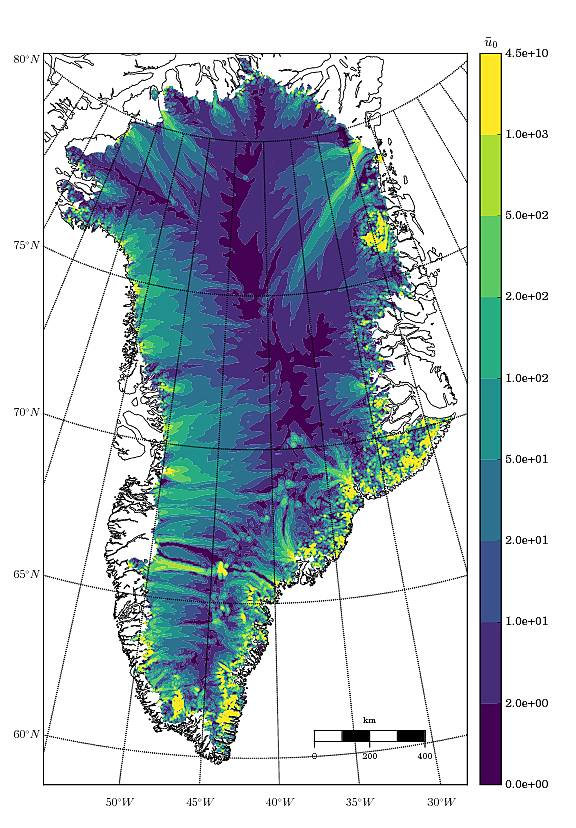
\includegraphics[width=\linewidth]{images/balance_velocity/greenland/d_U_ob/Ubar_5H_kappa_0_SUPG.jpg}
  \caption{$\kappa = 0$, SUPG.}
  \label{greenland_bv_image_d_U_ob_kappa_0_SUPG}
  \end{subfigure}
  \begin{subfigure}[b]{0.25\linewidth}
    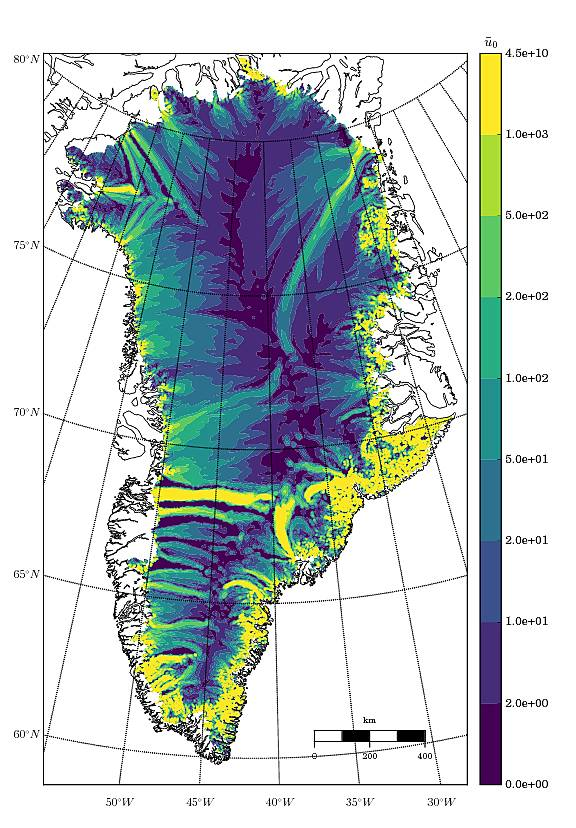
\includegraphics[width=\linewidth]{images/balance_velocity/greenland/d_U_ob/Ubar_5H_kappa_0_SSM.jpg}
  \caption{$\kappa = 0$, SSM.}
  \label{greenland_bv_image_d_U_ob_kappa_5_SSM}
  \end{subfigure}

  \begin{subfigure}[b]{0.25\linewidth}
    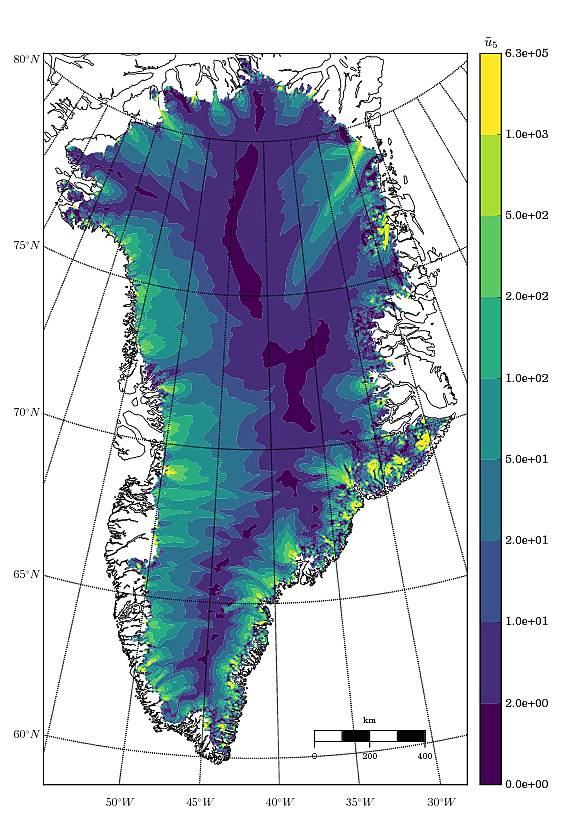
\includegraphics[width=\linewidth]{images/balance_velocity/greenland/d_U_ob/Ubar_5H_kappa_5_GLS.jpg}
  \caption{$\kappa = 5$, GLS.}
  \label{greenland_bv_image_d_U_ob_kappa_5_GLS}
  \end{subfigure}
  \begin{subfigure}[b]{0.25\linewidth}
    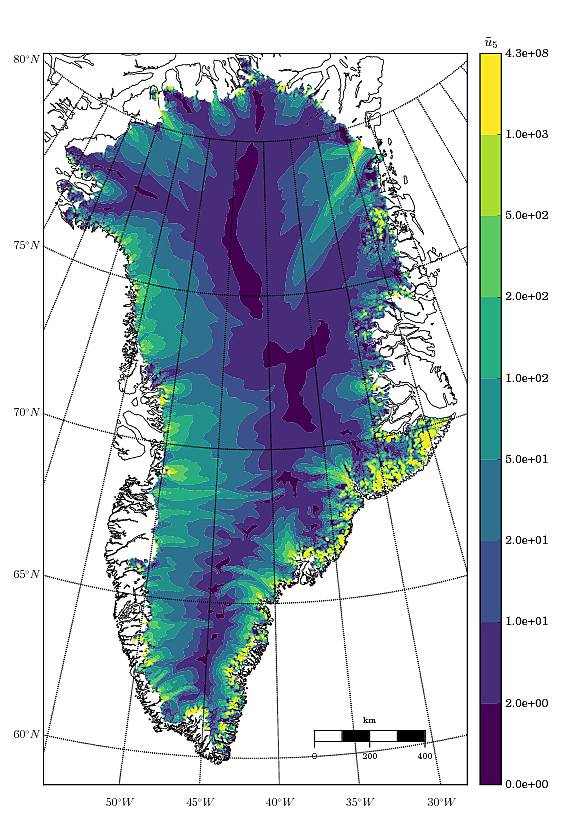
\includegraphics[width=\linewidth]{images/balance_velocity/greenland/d_U_ob/Ubar_5H_kappa_5_SUPG.jpg}
  \caption{$\kappa = 5$, SUPG.}
  \label{greenland_bv_image_d_U_ob_kappa_5_SUPG}
  \end{subfigure}
  \begin{subfigure}[b]{0.25\linewidth}
    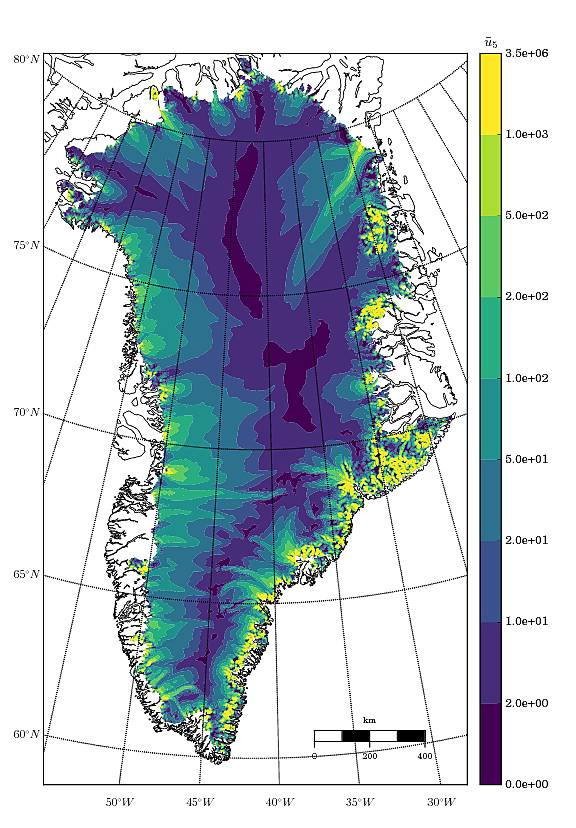
\includegraphics[width=\linewidth]{images/balance_velocity/greenland/d_U_ob/Ubar_5H_kappa_5_SSM.jpg}
  \caption{$\kappa = 5$, SSM.}
  \label{greenland_bv_image_d_U_ob_kappa_5_SSM}
  \end{subfigure}

  \begin{subfigure}[b]{0.25\linewidth}
    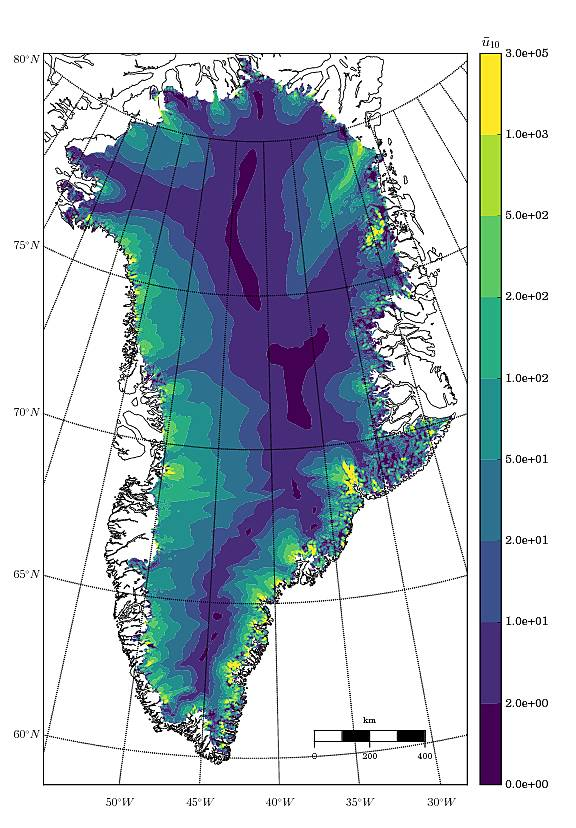
\includegraphics[width=\linewidth]{images/balance_velocity/greenland/d_U_ob/Ubar_5H_kappa_10_GLS.jpg}
  \caption{$\kappa = 10$, GLS.}
  \label{greenland_bv_image_d_U_ob_kappa_10_GLS}
  \end{subfigure}
  \begin{subfigure}[b]{0.25\linewidth}
    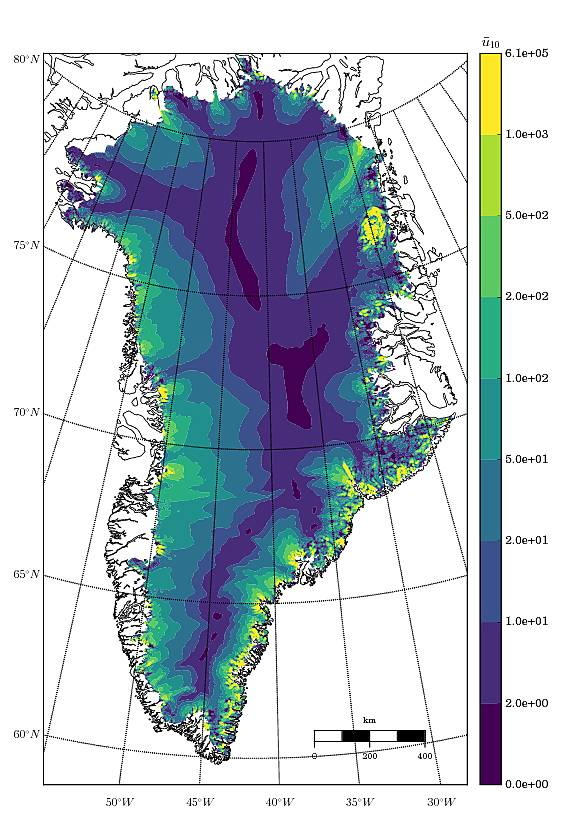
\includegraphics[width=\linewidth]{images/balance_velocity/greenland/d_U_ob/Ubar_5H_kappa_10_SUPG.jpg}
  \caption{$\kappa = 10$, SUPG.}
  \label{greenland_bv_image_d_U_ob_kappa_10_SUPG}
  \end{subfigure}
  \begin{subfigure}[b]{0.25\linewidth}
    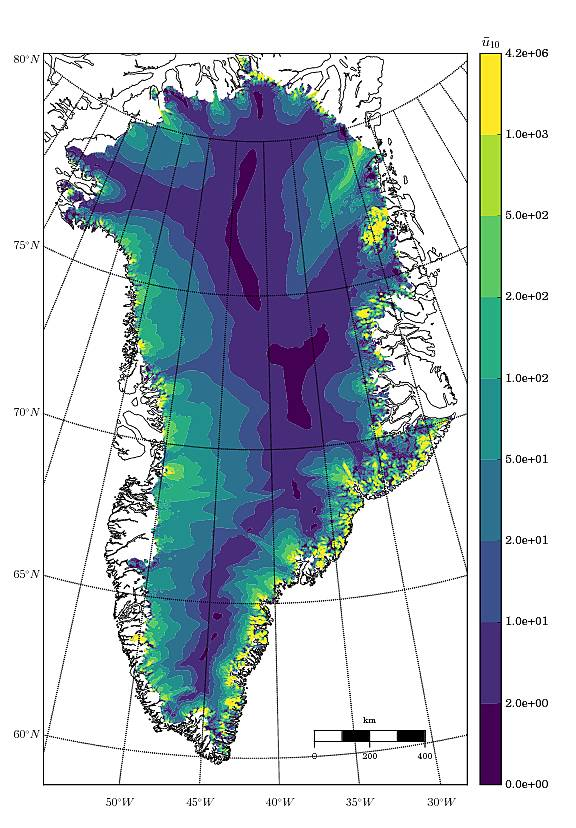
\includegraphics[width=\linewidth]{images/balance_velocity/greenland/d_U_ob/Ubar_5H_kappa_10_SSM.jpg}
  \caption{$\kappa = 10$, SSM.}
  \label{greenland_bv_image_d_U_ob_kappa_10_SSM}
  \end{subfigure}
 
  \caption[Greenland balance-velocity with $\mathbf{d}^{\text{data}} = \mathbf{u}_{ob}$.]{Balance velocity $\bar{u}$ derived over Greenland with direction of flow imposed in the direction of surface velocity observations $\rankone{u}_{ob}$, where smoothing radius $\kappa$ varies as indicated.  The columns vary according to stabilization used; either Galerkin/least-squares (GLS) stabilization \cref{bv_gls_operator}, streamline-upwind/Petrov-Galerkin (SUPG) stabilization \cref{bv_supg_operator}, or subgrid-scale-model (SSM) stabilization \cref{bv_ssm_operator} in variational form \cref{balance_velocity_weak_problem}. \newline}

  \label{greenland_bv_image_d_U_ob}

\end{figure*}

%===============================================================================

\begin{figure*}
  
  \centering 

  \begin{subfigure}[b]{0.25\linewidth}
    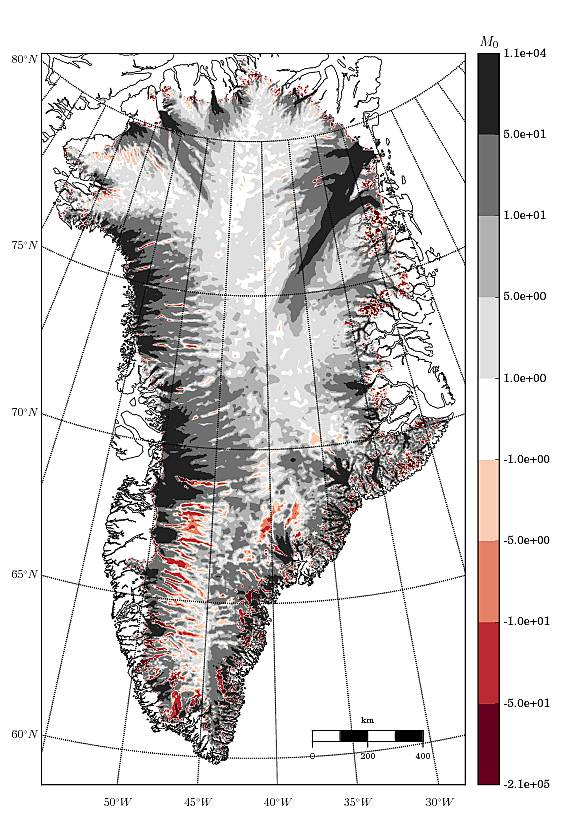
\includegraphics[width=\linewidth]{images/balance_velocity/greenland/misfit_5H_kappa_0_GLS.jpg}
  \caption{$\kappa = 0$, GLS.}
  \label{greenland_bv_image_kappa_0_GLS_misfit}
  \end{subfigure}
  \begin{subfigure}[b]{0.25\linewidth}
    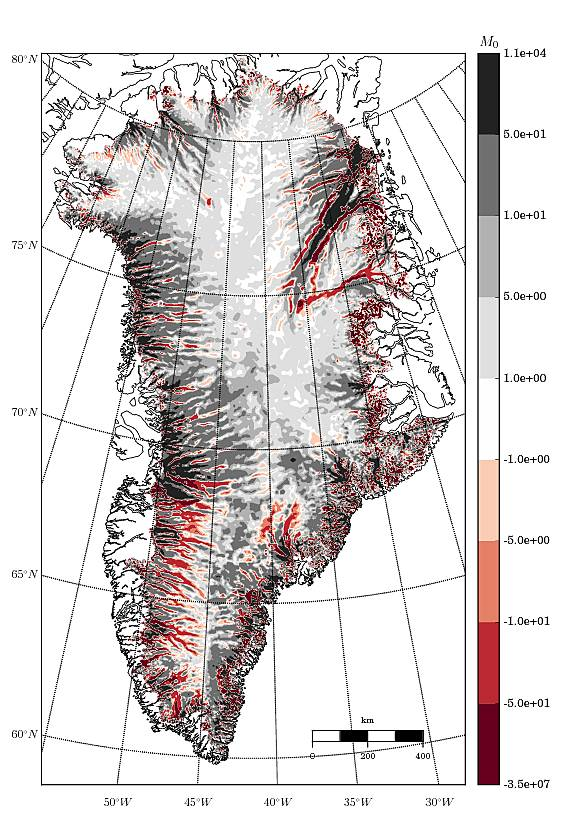
\includegraphics[width=\linewidth]{images/balance_velocity/greenland/misfit_5H_kappa_0_SUPG.jpg}
  \caption{$\kappa = 0$, SUPG.}
  \label{greenland_bv_image_kappa_0_SUPG_misfit}
  \end{subfigure}
  \begin{subfigure}[b]{0.25\linewidth}
    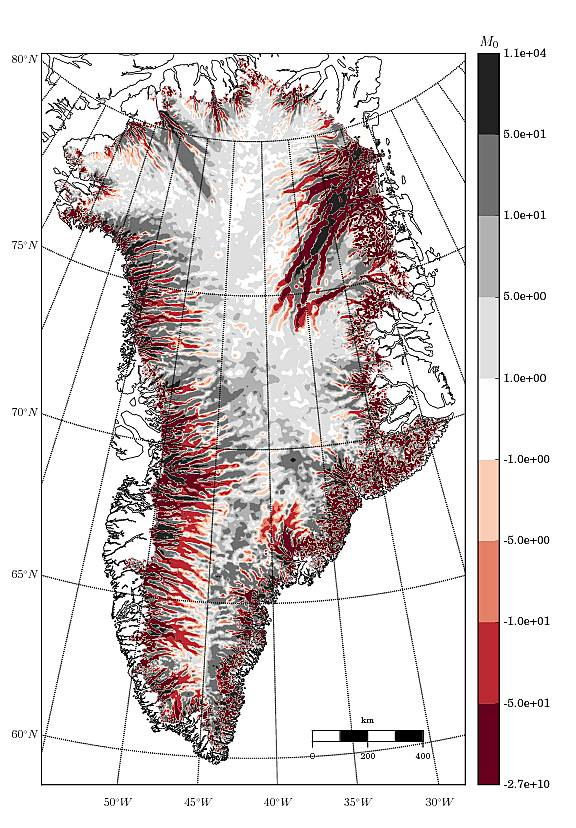
\includegraphics[width=\linewidth]{images/balance_velocity/greenland/misfit_5H_kappa_0_SSM.jpg}
  \caption{$\kappa = 0$, SSM.}
  \label{greenland_bv_image_kappa_5_SSM_misfit}
  \end{subfigure}

  \begin{subfigure}[b]{0.25\linewidth}
    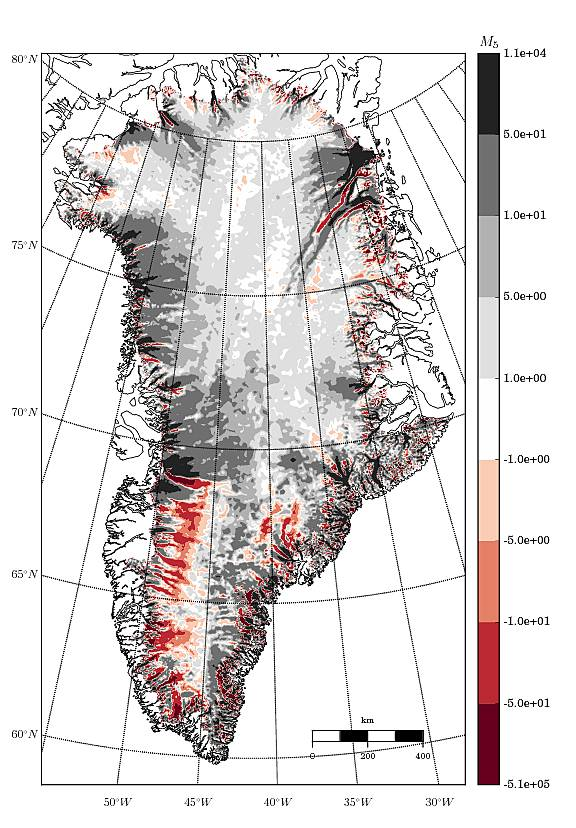
\includegraphics[width=\linewidth]{images/balance_velocity/greenland/misfit_5H_kappa_5_GLS.jpg}
  \caption{$\kappa = 5$, GLS.}
  \label{greenland_bv_image_kappa_5_GLS_misfit}
  \end{subfigure}
  \begin{subfigure}[b]{0.25\linewidth}
    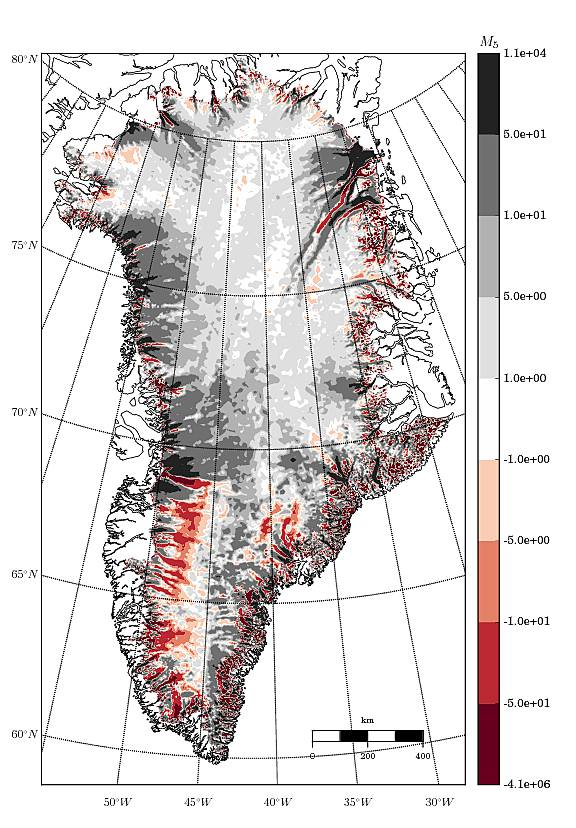
\includegraphics[width=\linewidth]{images/balance_velocity/greenland/misfit_5H_kappa_5_SUPG.jpg}
  \caption{$\kappa = 5$, SUPG.}
  \label{greenland_bv_image_kappa_5_SUPG_misfit}
  \end{subfigure}
  \begin{subfigure}[b]{0.25\linewidth}
    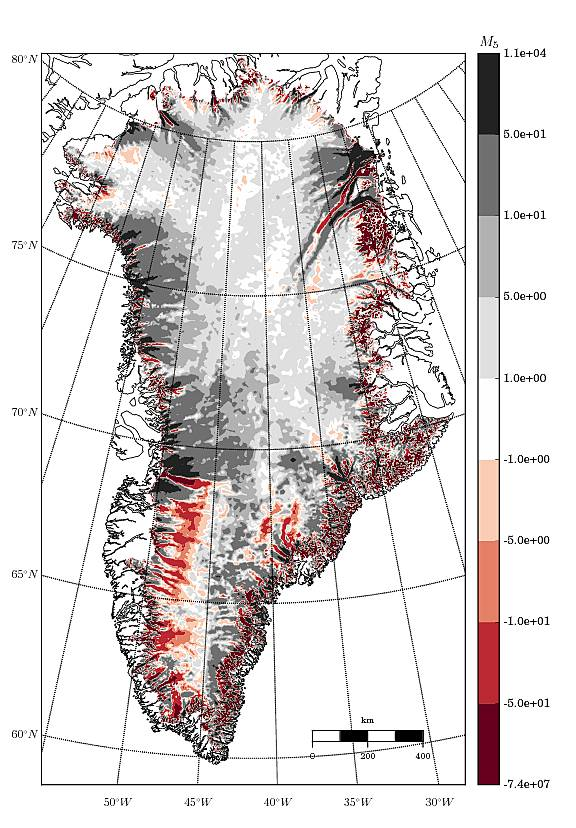
\includegraphics[width=\linewidth]{images/balance_velocity/greenland/misfit_5H_kappa_5_SSM.jpg}
  \caption{$\kappa = 5$, SSM.}
  \label{greenland_bv_image_kappa_5_SSM_misfit}
  \end{subfigure}

  \begin{subfigure}[b]{0.25\linewidth}
    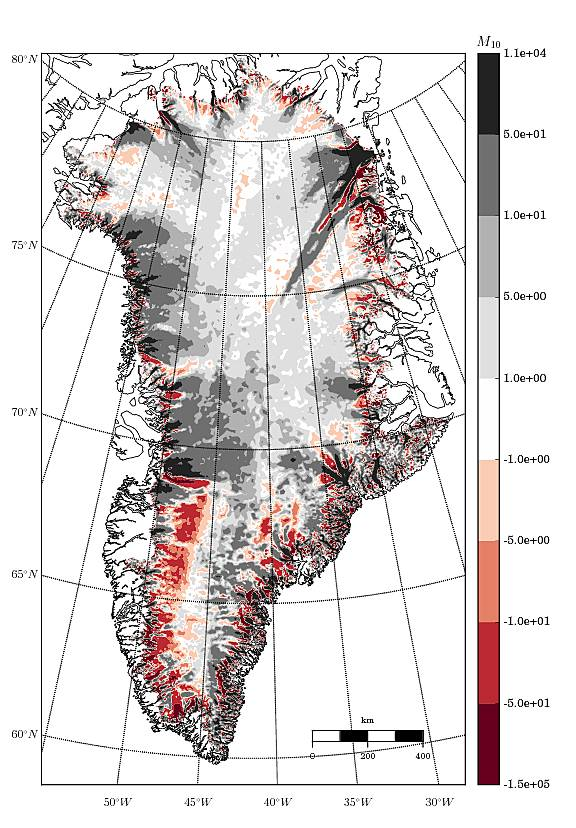
\includegraphics[width=\linewidth]{images/balance_velocity/greenland/misfit_5H_kappa_10_GLS.jpg}
  \caption{$\kappa = 10$, GLS.}
  \label{greenland_bv_image_kappa_10_GLS_misfit}
  \end{subfigure}
  \begin{subfigure}[b]{0.25\linewidth}
    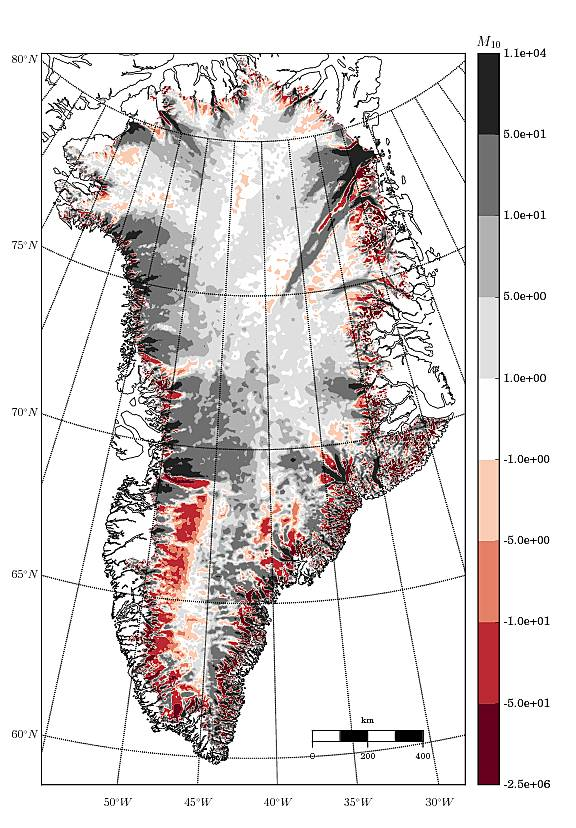
\includegraphics[width=\linewidth]{images/balance_velocity/greenland/misfit_5H_kappa_10_SUPG.jpg}
  \caption{$\kappa = 10$, SUPG.}
  \label{greenland_bv_image_kappa_10_SUPG_misfit}
  \end{subfigure}
  \begin{subfigure}[b]{0.25\linewidth}
    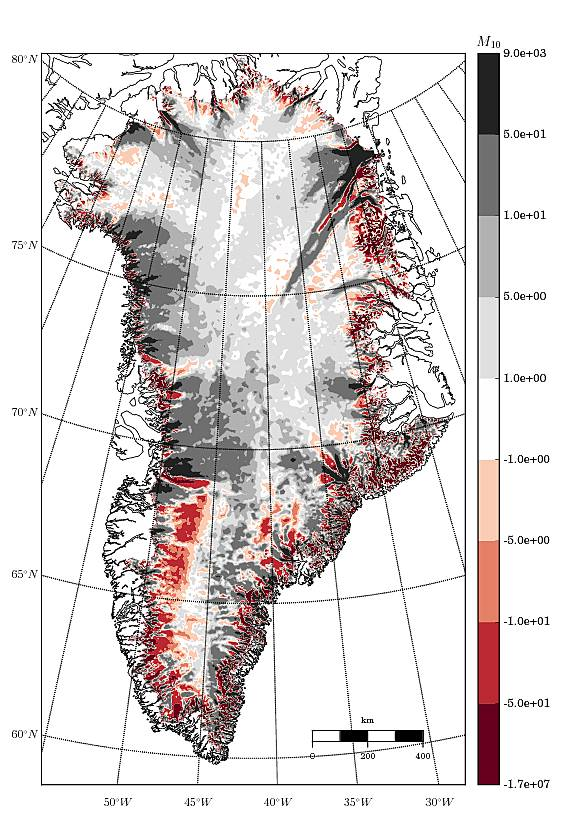
\includegraphics[width=\linewidth]{images/balance_velocity/greenland/misfit_5H_kappa_10_SSM.jpg}
  \caption{$\kappa = 10$, SSM.}
  \label{greenland_bv_image_kappa_10_SSM_misfit}
  \end{subfigure}
 
  \caption[Greenland balance-velocity misfit with $\mathbf{d}^{\text{data}} = -\nabla S$.]{Difference $\Vert \rankone{u}_{ob} \Vert - \bar{u}$ between balance velocity $\bar{u}$ and the magnitude of the observed surface velocity $\rankone{u}_{ob}$ derived over Greenland with imposed direction of flow down the surface gradient $\nabla S$, where smoothing radius $\kappa$ varies as indicated.  The columns vary according to stabilization used; either Galerkin/least-squares (GLS) stabilization \cref{bv_gls_operator}, streamline-upwind/Petrov-Galerkin (SUPG) stabilization \cref{bv_supg_operator}, or subgrid-scale-model (SSM) stabilization \cref{bv_ssm_operator} in variational form \cref{balance_velocity_weak_problem}.}

  \label{greenland_bv_image_misfit}

\end{figure*}

%===============================================================================

\begin{figure*}
  
  \centering 

  \begin{subfigure}[b]{0.25\linewidth}
    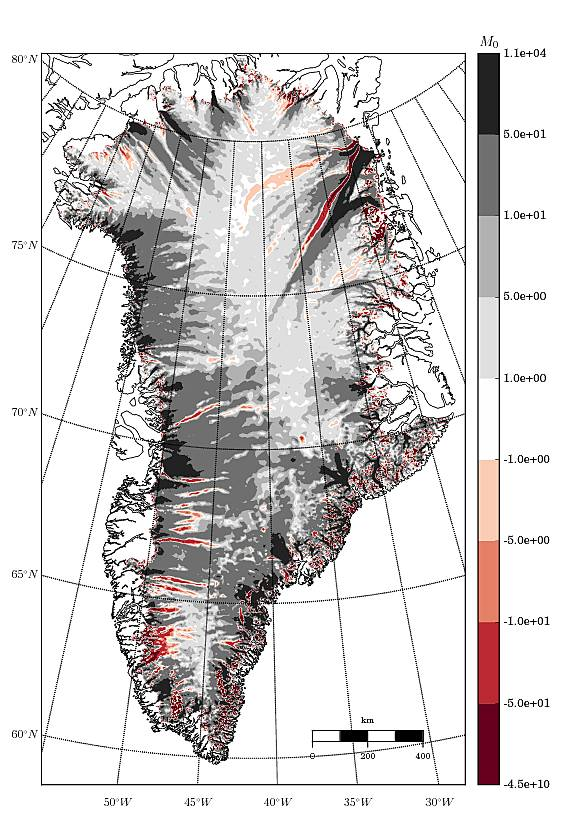
\includegraphics[width=\linewidth]{images/balance_velocity/greenland/d_U_ob/misfit_5H_kappa_0_GLS.jpg}
  \caption{$\kappa = 0$, GLS.}
  \label{greenland_bv_image_d_U_ob_kappa_0_GLS_misfit}
  \end{subfigure}
  \begin{subfigure}[b]{0.25\linewidth}
    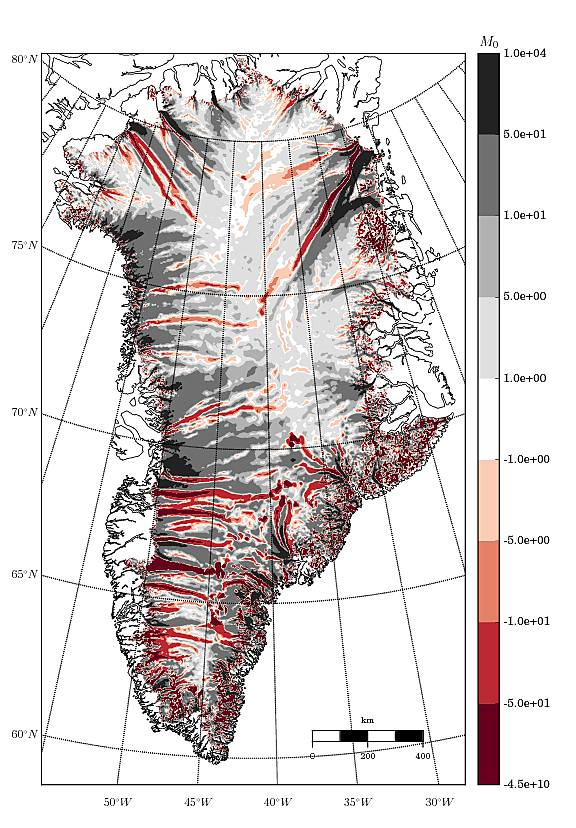
\includegraphics[width=\linewidth]{images/balance_velocity/greenland/d_U_ob/misfit_5H_kappa_0_SUPG.jpg}
  \caption{$\kappa = 0$, SUPG.}
  \label{greenland_bv_image_d_U_ob_kappa_0_SUPG_misfit}
  \end{subfigure}
  \begin{subfigure}[b]{0.25\linewidth}
    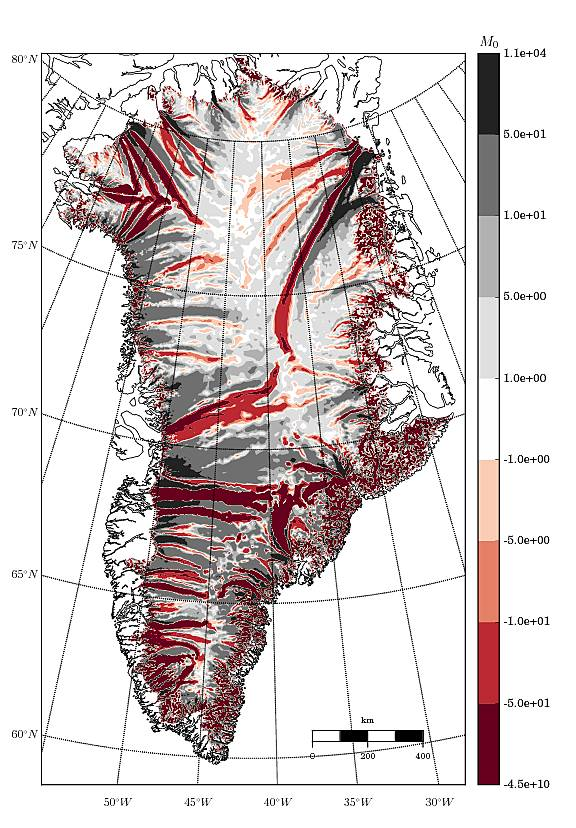
\includegraphics[width=\linewidth]{images/balance_velocity/greenland/d_U_ob/misfit_5H_kappa_0_SSM.jpg}
  \caption{$\kappa = 0$, SSM.}
  \label{greenland_bv_image_d_U_ob_kappa_5_SSM_misfit}
  \end{subfigure}

  \begin{subfigure}[b]{0.25\linewidth}
    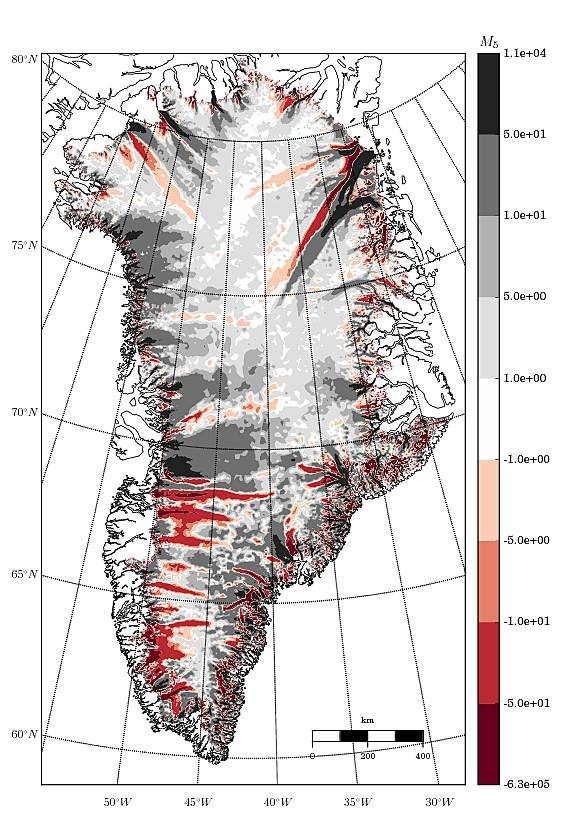
\includegraphics[width=\linewidth]{images/balance_velocity/greenland/d_U_ob/misfit_5H_kappa_5_GLS.jpg}
  \caption{$\kappa = 5$, GLS.}
  \label{greenland_bv_image_d_U_ob_kappa_5_GLS_misfit}
  \end{subfigure}
  \begin{subfigure}[b]{0.25\linewidth}
    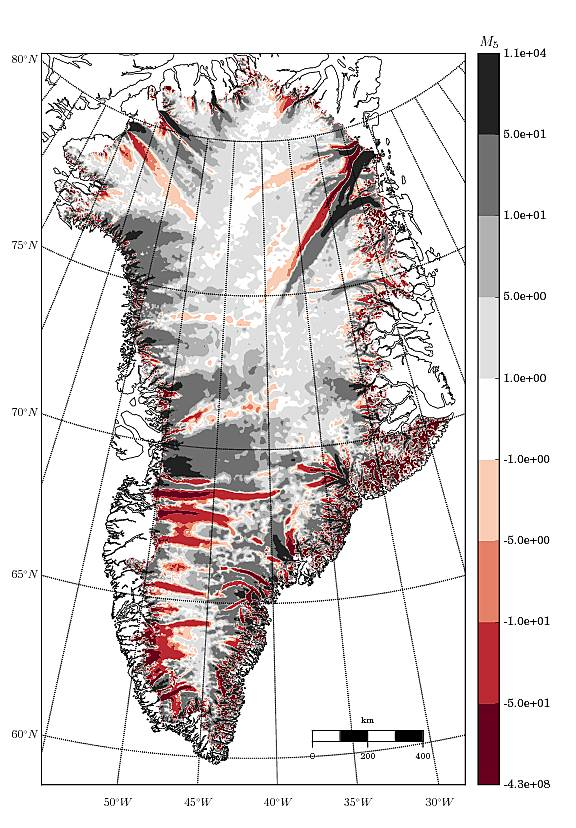
\includegraphics[width=\linewidth]{images/balance_velocity/greenland/d_U_ob/misfit_5H_kappa_5_SUPG.jpg}
  \caption{$\kappa = 5$, SUPG.}
  \label{greenland_bv_image_d_U_ob_kappa_5_SUPG_misfit}
  \end{subfigure}
  \begin{subfigure}[b]{0.25\linewidth}
    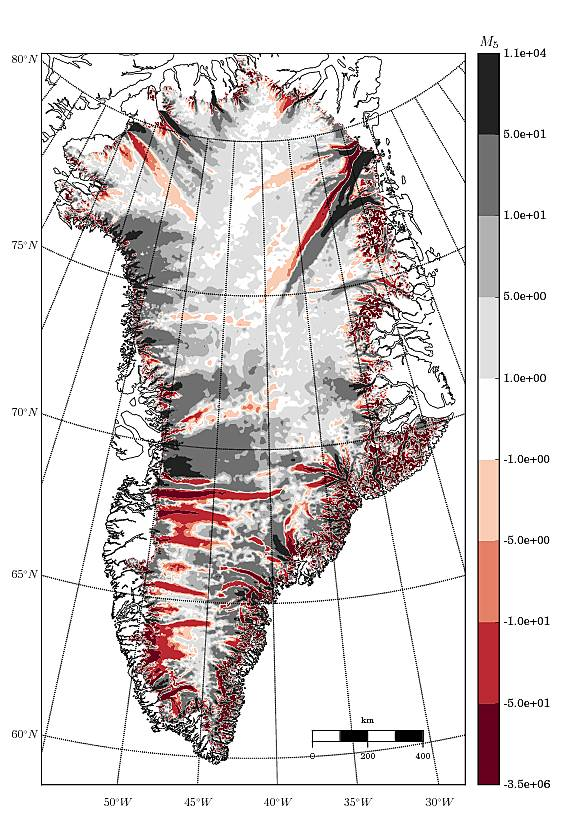
\includegraphics[width=\linewidth]{images/balance_velocity/greenland/d_U_ob/misfit_5H_kappa_5_SSM.jpg}
  \caption{$\kappa = 5$, SSM.}
  \label{greenland_bv_image_d_U_ob_kappa_5_SSM_misfit}
  \end{subfigure}

  \begin{subfigure}[b]{0.25\linewidth}
    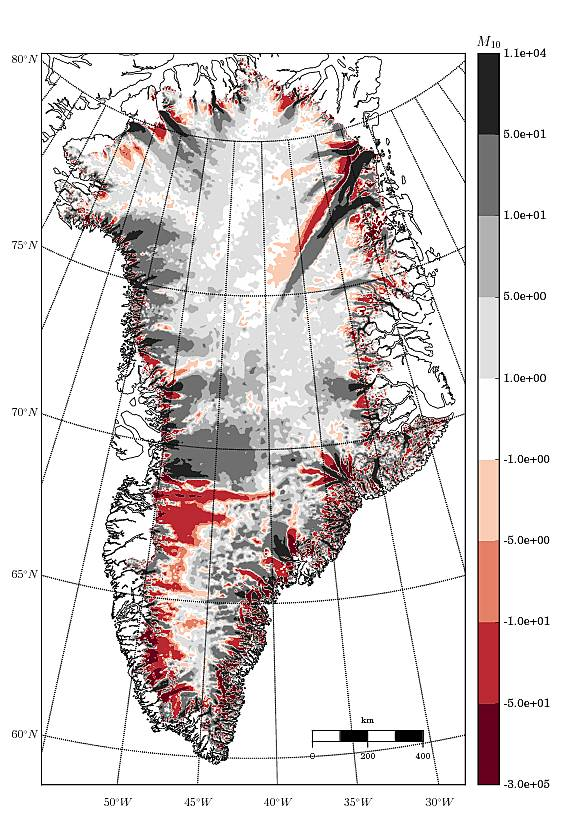
\includegraphics[width=\linewidth]{images/balance_velocity/greenland/d_U_ob/misfit_5H_kappa_10_GLS.jpg}
  \caption{$\kappa = 10$, GLS.}
  \label{greenland_bv_image_d_U_ob_kappa_10_GLS_misfit}
  \end{subfigure}
  \begin{subfigure}[b]{0.25\linewidth}
    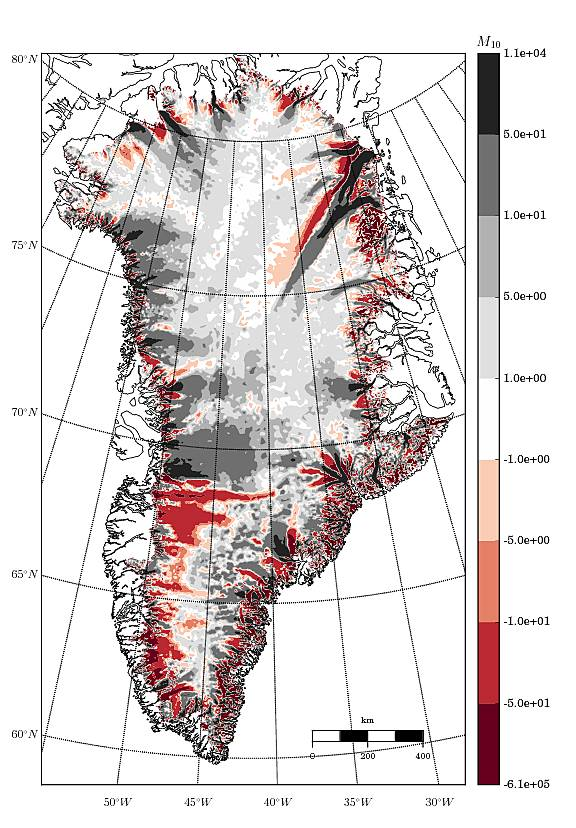
\includegraphics[width=\linewidth]{images/balance_velocity/greenland/d_U_ob/misfit_5H_kappa_10_SUPG.jpg}
  \caption{$\kappa = 10$, SUPG.}
  \label{greenland_bv_image_d_U_ob_kappa_10_SUPG_misfit}
  \end{subfigure}
  \begin{subfigure}[b]{0.25\linewidth}
    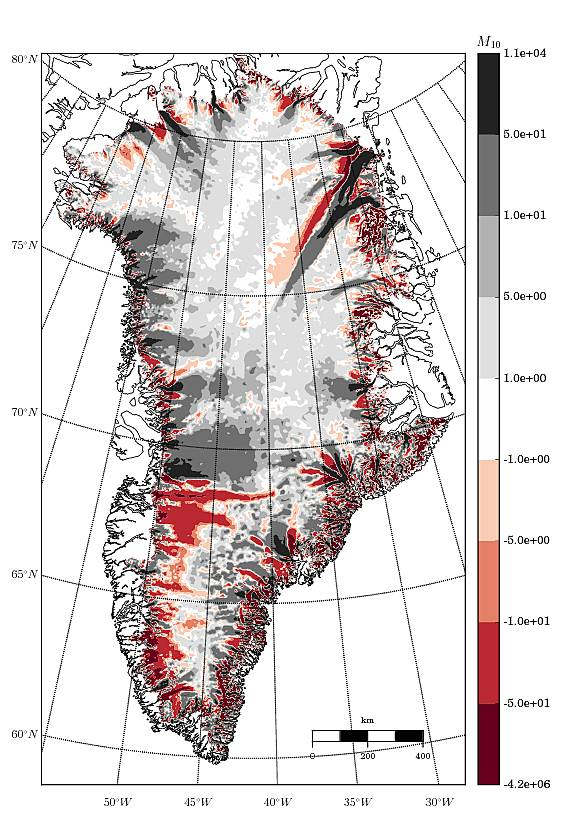
\includegraphics[width=\linewidth]{images/balance_velocity/greenland/d_U_ob/misfit_5H_kappa_10_SSM.jpg}
  \caption{$\kappa = 10$, SSM.}
  \label{greenland_bv_image_d_U_ob_kappa_10_SSM_misfit}
  \end{subfigure}
 
  \caption[Greenland balance-velocity misfit with $\mathbf{d}^{\text{data}} = \mathbf{u}_{ob}$.]{Difference $\Vert \rankone{u}_{ob} \Vert - \bar{u}$ between balance velocity $\bar{u}$ and the magnitude of the observed surface velocity $\rankone{u}_{ob}$ derived over Greenland with imposed direction of flow in the direction of surface velocity observations $\rankone{u}_{ob}$, where smoothing radius $\kappa$ varies as indicated.  The columns vary according to stabilization used; either Galerkin/least-squares (GLS) stabilization \cref{bv_gls_operator}, streamline-upwind/Petrov-Galerkin (SUPG) stabilization \cref{bv_supg_operator}, or subgrid-scale-model (SSM) stabilization \cref{bv_ssm_operator} in variational form \cref{balance_velocity_weak_problem}.}

  \label{greenland_bv_image_d_U_ob_misfit}

\end{figure*}

%===============================================================================

\begin{figure*}
  \centering
    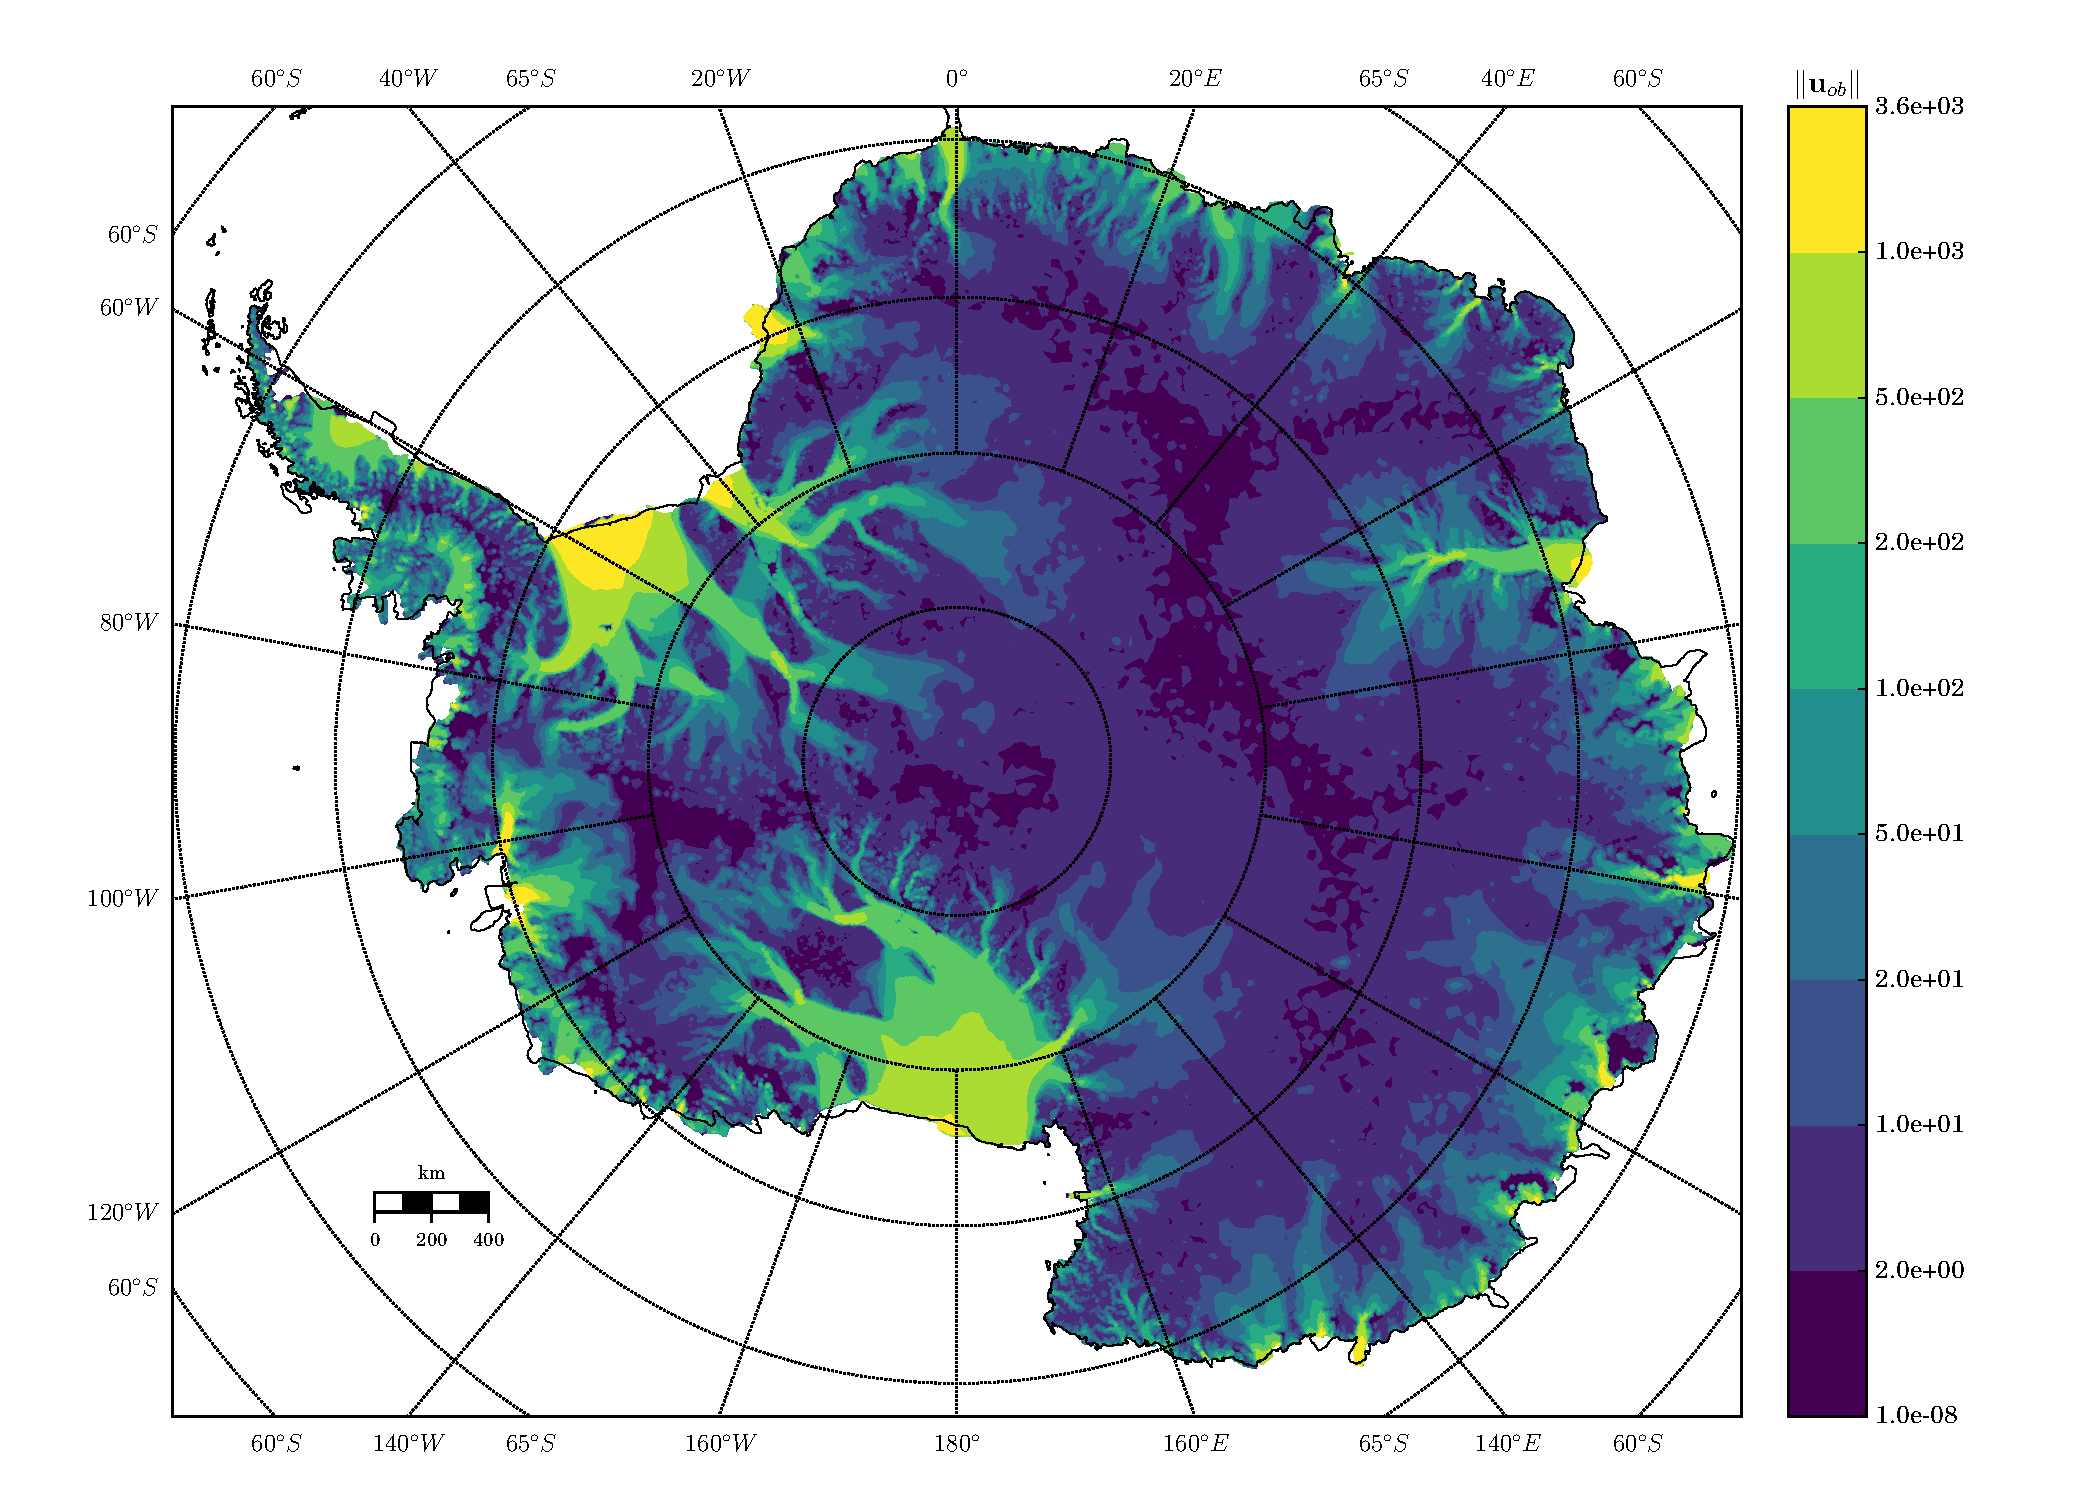
\includegraphics[width=\linewidth]{images/balance_velocity/antarctica/U_ob.pdf}
  \caption[Antarctica surface velocity magnitude]{Surface velocity magnitude of Antarctica as provided by \citet{rignot_2011a, rignot_2011}.}
  \label{antarctica_u_ob_image}
\end{figure*}

%===============================================================================

\begin{figure*}

  \centering

  \begin{subfigure}[b]{0.45\linewidth}
    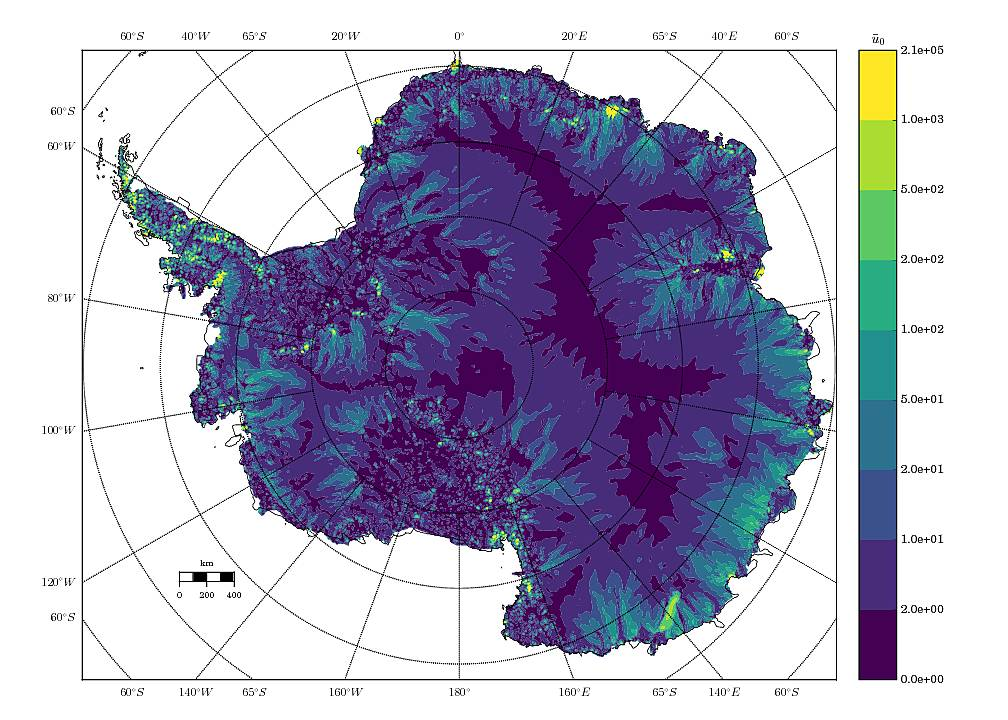
\includegraphics[width=\linewidth]{images/balance_velocity/antarctica/Ubar_10H_kappa_0_GLS.jpg}
  \caption{$\kappa = 0$, GLS.}
  \label{antarctica_bv_image_kappa_0_GLS}
  \end{subfigure}
  \begin{subfigure}[b]{0.45\linewidth}
    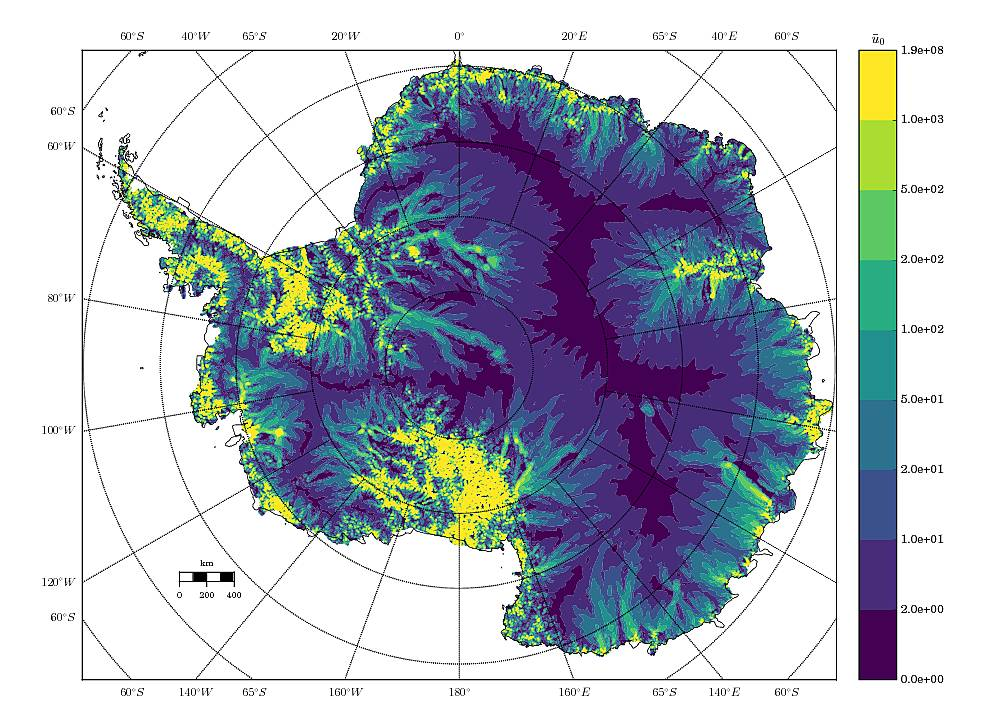
\includegraphics[width=\linewidth]{images/balance_velocity/antarctica/Ubar_10H_kappa_0_SUPG.jpg}
  \caption{$\kappa = 0$, SUPG.}
  \label{antarctica_bv_image_kappa_0_SUPG}
  \end{subfigure}

  \begin{subfigure}[b]{0.45\linewidth}
    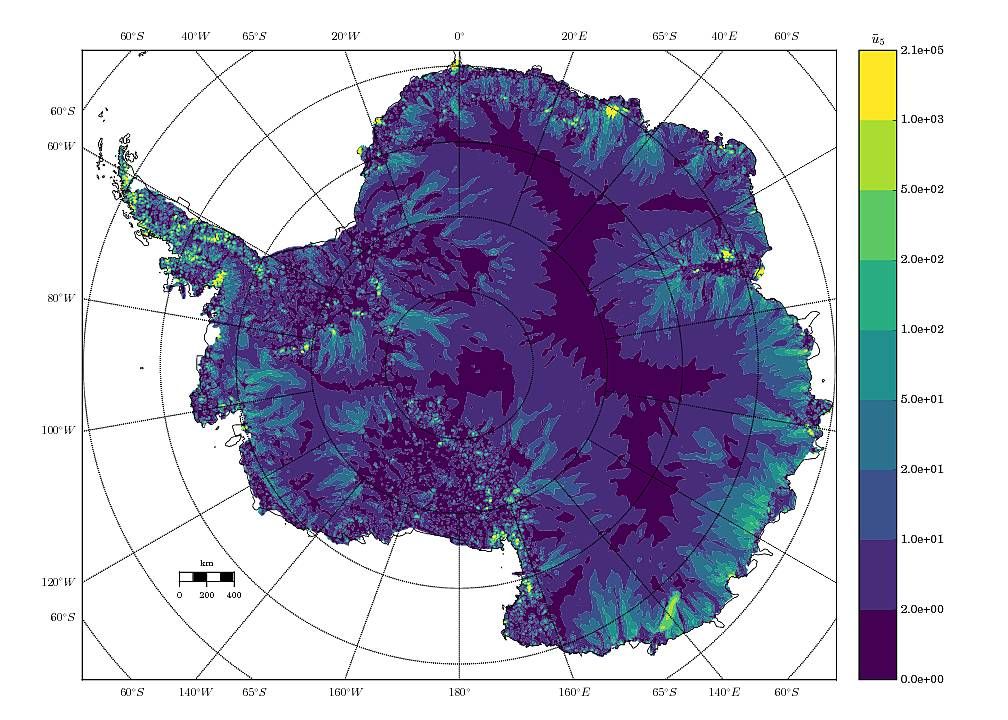
\includegraphics[width=\linewidth]{images/balance_velocity/antarctica/Ubar_10H_kappa_5_GLS.jpg}
  \caption{$\kappa = 5$, GLS.}
  \label{antarctica_bv_image_kappa_5_GLS}
  \end{subfigure}
  \begin{subfigure}[b]{0.45\linewidth}
    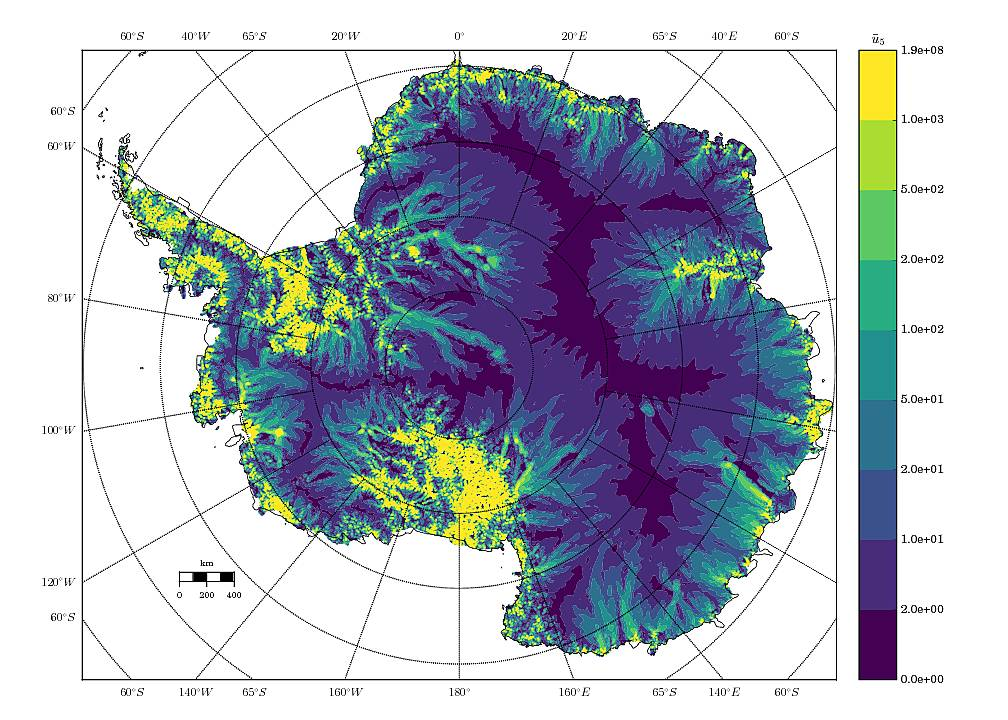
\includegraphics[width=\linewidth]{images/balance_velocity/antarctica/Ubar_10H_kappa_5_SUPG.jpg}
  \caption{$\kappa = 5$, SUPG.}
  \label{antarctica_bv_image_kappa_5_SUPG}
  \end{subfigure}

  \begin{subfigure}[b]{0.45\linewidth}
    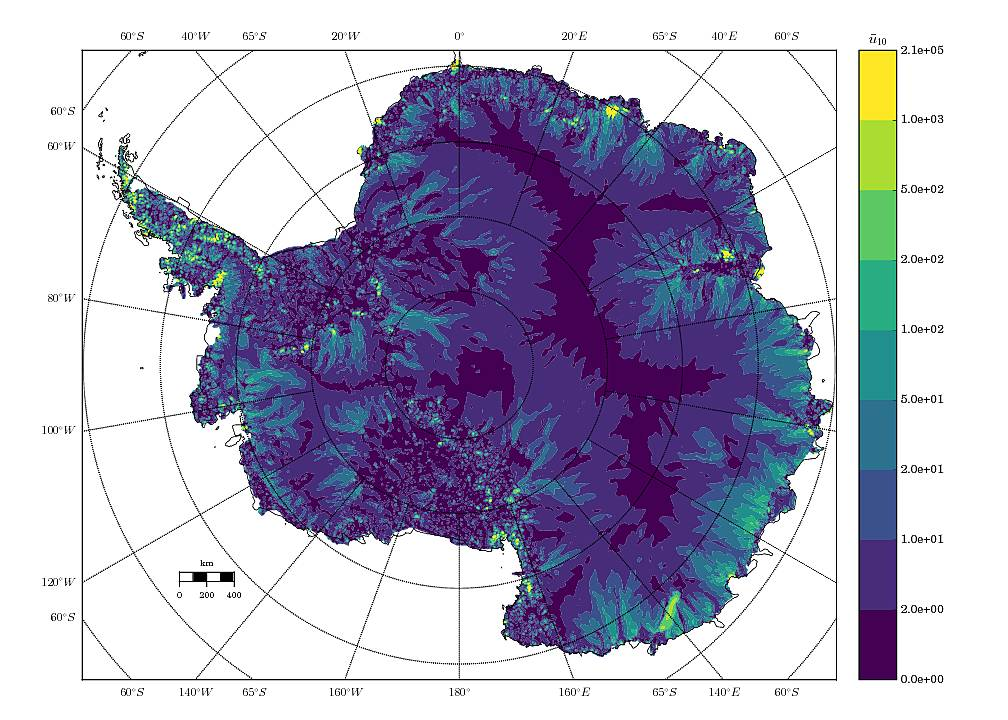
\includegraphics[width=\linewidth]{images/balance_velocity/antarctica/Ubar_10H_kappa_10_GLS.jpg}
  \caption{$\kappa = 10$, GLS.}
  \label{antarctica_bv_image_kappa_10_GLS}
  \end{subfigure}
  \begin{subfigure}[b]{0.45\linewidth}
    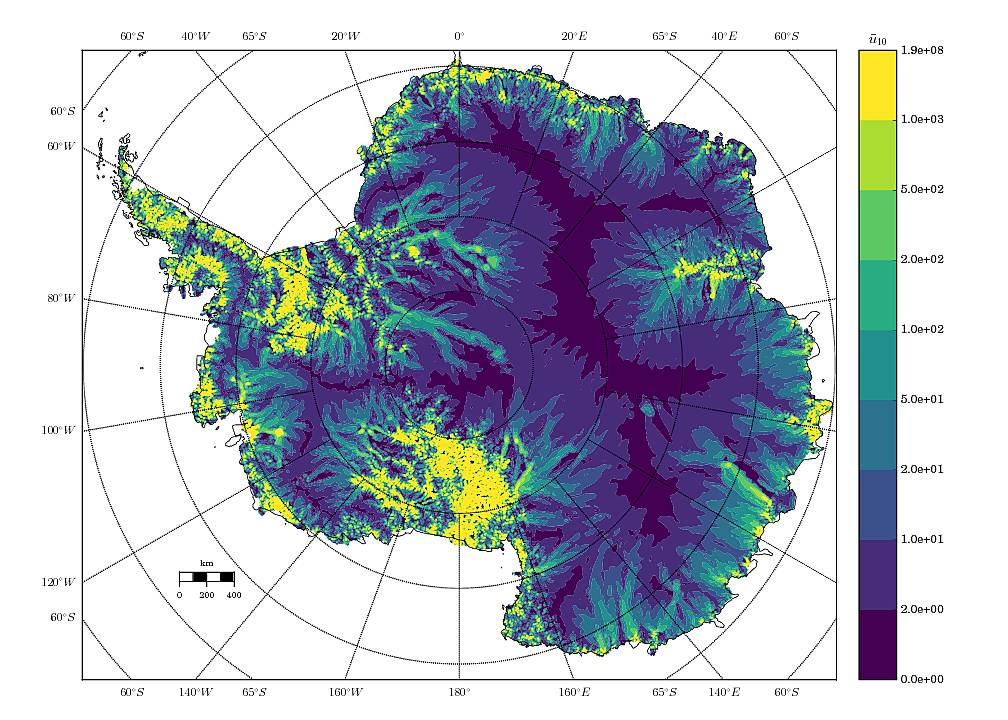
\includegraphics[width=\linewidth]{images/balance_velocity/antarctica/Ubar_10H_kappa_10_SUPG.jpg}
  \caption{$\kappa = 10$, SUPG.}
  \label{antarctica_bv_image_kappa_10_SUPG}
  \end{subfigure}
  
  \caption[Antarctica balance-velocity with $\mathbf{d}^{\text{data}} = -\nabla S$.]{Balance velocity $\bar{u}$ derived over Antarctica with imposed direction of flow down the surface gradient $\nabla S$, where smoothing radius $\kappa$ varies as indicated.  The columns vary according to stabilization used; either Galerkin/least-squares (GLS) stabilization \cref{bv_gls_operator} or streamline-upwind/Petrov-Galerkin (SUPG) stabilization \cref{bv_supg_operator} in variational form \cref{balance_velocity_weak_problem}.  Results using subgrid-scale-model stabilization \cref{bv_ssm_operator} (not shown) appeared more unstable than the (SUPG) method. \newline \newline}

  \label{antarctica_bv_image}
  
\end{figure*}

%===============================================================================

\begin{figure*}

  \centering

  \begin{subfigure}[b]{0.45\linewidth}
    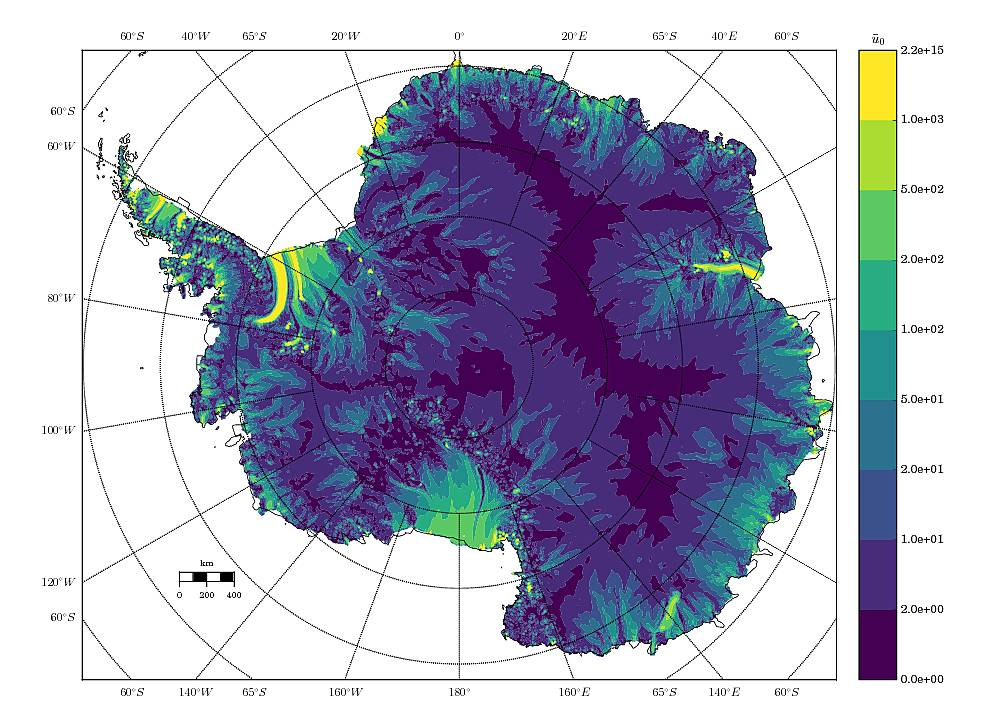
\includegraphics[width=\linewidth]{images/balance_velocity/antarctica/d_U_ob_S/Ubar_10H_kappa_0_GLS.jpg}
  \caption{$\kappa = 0$, GLS.}
  \label{antarctica_bv_image_kappa_0_GLS_U_ob_S}
  \end{subfigure}
  \begin{subfigure}[b]{0.45\linewidth}
    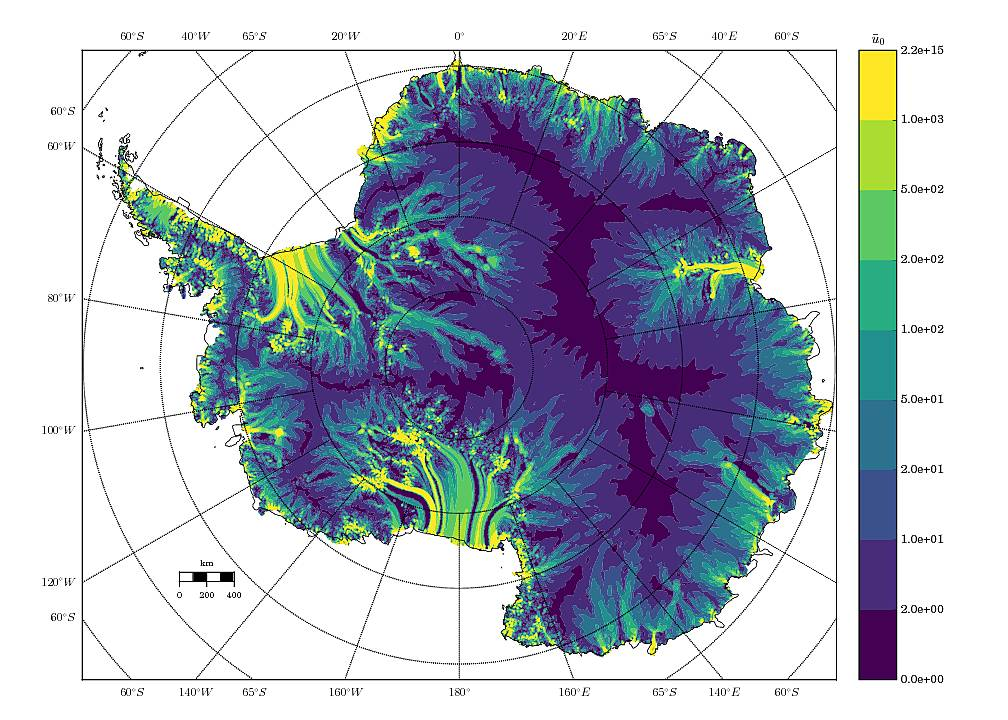
\includegraphics[width=\linewidth]{images/balance_velocity/antarctica/d_U_ob_S/Ubar_10H_kappa_0_SUPG.jpg}
  \caption{$\kappa = 0$, SUPG.}
  \label{antarctica_bv_image_kappa_0_SUPG_U_ob_S}
  \end{subfigure}

  \begin{subfigure}[b]{0.45\linewidth}
    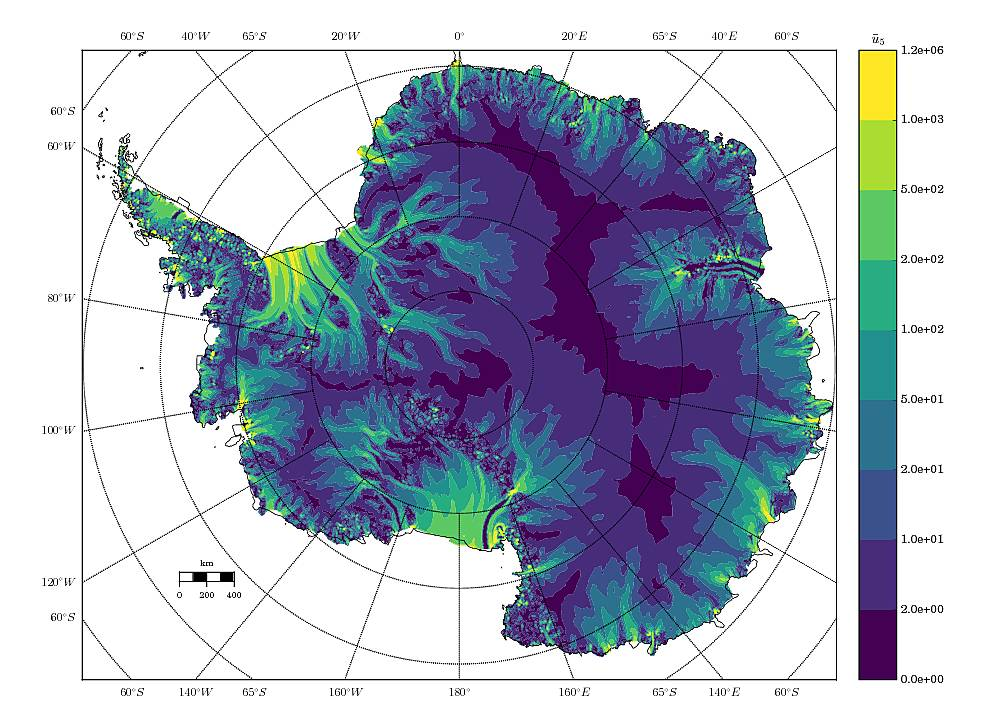
\includegraphics[width=\linewidth]{images/balance_velocity/antarctica/d_U_ob_S/Ubar_10H_kappa_5_GLS.jpg}
  \caption{$\kappa = 5$, GLS.}
  \label{antarctica_bv_image_kappa_5_GLS_U_ob_S}
  \end{subfigure}
  \begin{subfigure}[b]{0.45\linewidth}
    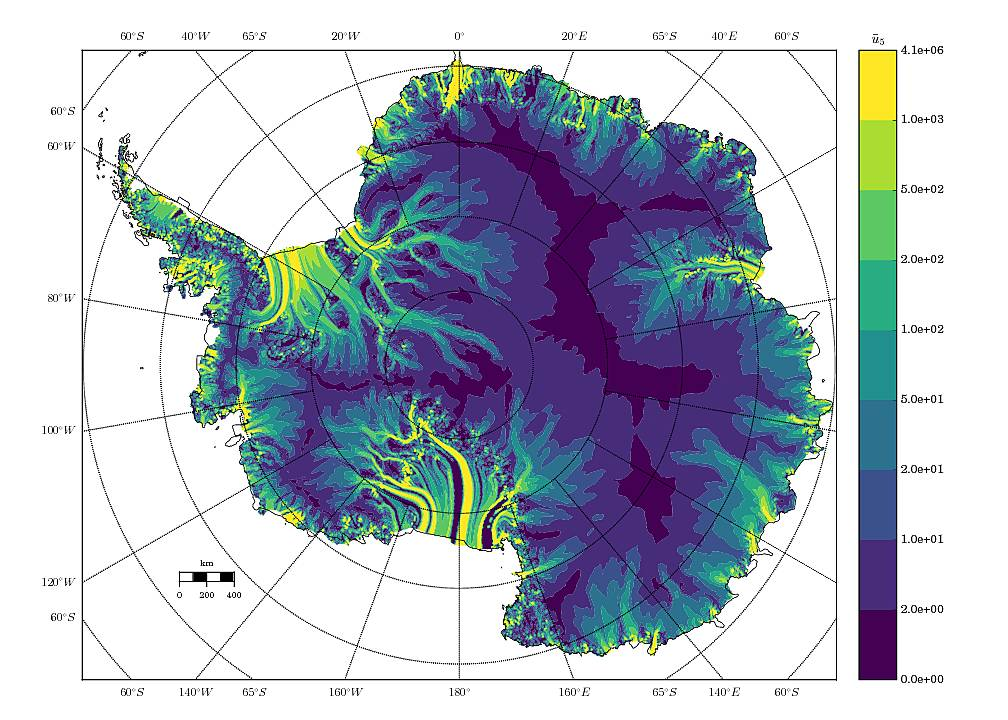
\includegraphics[width=\linewidth]{images/balance_velocity/antarctica/d_U_ob_S/Ubar_10H_kappa_5_SUPG.jpg}
  \caption{$\kappa = 5$, SUPG.}
  \label{antarctica_bv_image_kappa_5_SUPG_U_ob_S}
  \end{subfigure}

  \begin{subfigure}[b]{0.45\linewidth}
    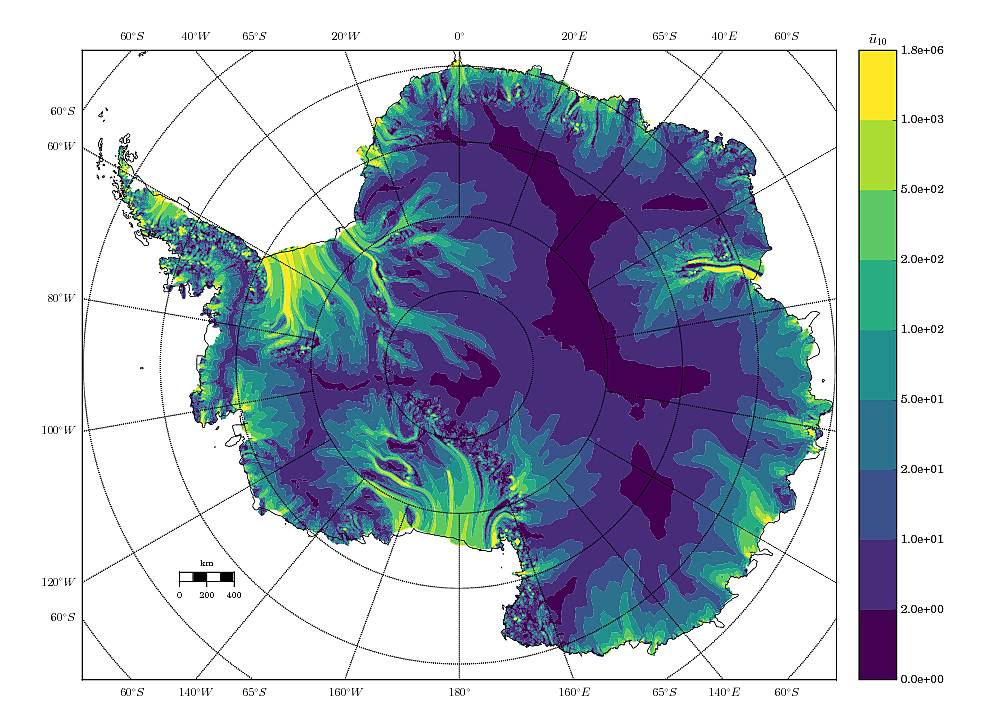
\includegraphics[width=\linewidth]{images/balance_velocity/antarctica/d_U_ob_S/Ubar_10H_kappa_10_GLS.jpg}
  \caption{$\kappa = 10$, GLS.}
  \label{antarctica_bv_image_kappa_5_GLS_U_ob_S}
  \end{subfigure}
  \begin{subfigure}[b]{0.45\linewidth}
    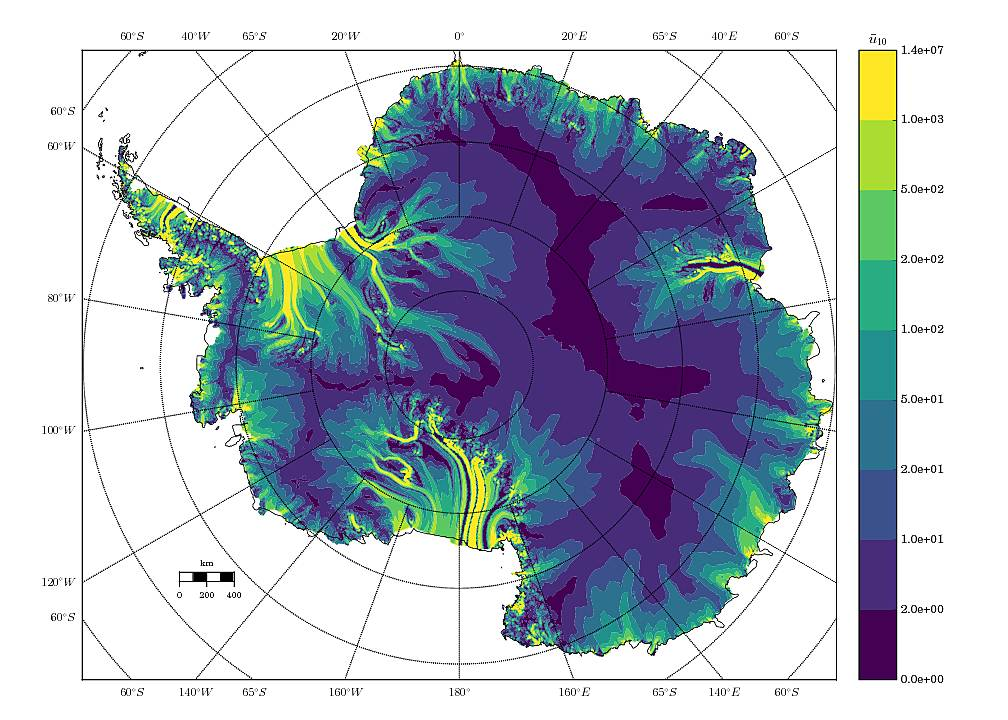
\includegraphics[width=\linewidth]{images/balance_velocity/antarctica/d_U_ob_S/Ubar_10H_kappa_10_SUPG.jpg}
  \caption{$\kappa = 10$, SUPG.}
  \label{antarctica_bv_image_kappa_5_SUPG_U_ob_S}
  \end{subfigure}
  
  \caption[Antarctica balance-velocity with $\mathbf{d}^{\text{data}} = \mathbf{u}_{ob}$ over shelves.]{Balance velocity $\bar{u}$ derived over Antarctica with imposed direction of flow down the surface gradient $\nabla S$ over grounded ice and in the direction of surface observations $\rankone{u}_{ob}$ over floating ice, where smoothing radius $\kappa$ varies as indicated.  The columns vary according to stabilization used; either Galerkin/least-squares (GLS) stabilization \cref{bv_gls_operator} or streamline-upwind/Petrov-Galerkin (SUPG) stabilization \cref{bv_supg_operator} in variational form \cref{balance_velocity_weak_problem}.  Results using subgrid-scale-model stabilization \cref{bv_ssm_operator} (not shown) appeared more unstable than the (SUPG) method. \newline}

  \label{antarctica_bv_image_U_ob_S}

\end{figure*}

%===============================================================================

\begin{figure*}

  \centering

  \begin{subfigure}[b]{0.45\linewidth}
    \includegraphics[width=\linewidth]{images/balance_velocity/antarctica/d_U_ob/Ubar_10H_kappa_0_GLS.jpg}
  \caption{$\kappa = 0$, GLS.}
  \label{antarctica_bv_image_d_U_ob_kappa_0_GLS}
  \end{subfigure}
  \begin{subfigure}[b]{0.45\linewidth}
    \includegraphics[width=\linewidth]{images/balance_velocity/antarctica/d_U_ob/Ubar_10H_kappa_0_SUPG.jpg}
  \caption{$\kappa = 0$, SUPG.}
  \label{antarctica_bv_image_d_U_ob_kappa_0_SUPG}
  \end{subfigure}

  \begin{subfigure}[b]{0.45\linewidth}
    \includegraphics[width=\linewidth]{images/balance_velocity/antarctica/d_U_ob/Ubar_10H_kappa_5_GLS.jpg}
  \caption{$\kappa = 5$, GLS.}
  \label{antarctica_bv_image_d_U_ob_kappa_5_GLS}
  \end{subfigure}
  \begin{subfigure}[b]{0.45\linewidth}
    \includegraphics[width=\linewidth]{images/balance_velocity/antarctica/d_U_ob/Ubar_10H_kappa_5_SUPG.jpg}
  \caption{$\kappa = 5$, SUPG.}
  \label{antarctica_bv_image_d_U_ob_kappa_5_SUPG}
  \end{subfigure}

  \begin{subfigure}[b]{0.45\linewidth}
    \includegraphics[width=\linewidth]{images/balance_velocity/antarctica/d_U_ob/Ubar_10H_kappa_10_GLS.jpg}
  \caption{$\kappa = 10$, GLS.}
  \label{antarctica_bv_image_d_U_ob_kappa_10_GLS}
  \end{subfigure}
  \begin{subfigure}[b]{0.45\linewidth}
    \includegraphics[width=\linewidth]{images/balance_velocity/antarctica/d_U_ob/Ubar_10H_kappa_10_SUPG.jpg}
  \caption{$\kappa = 10$, SUPG.}
  \label{antarctica_bv_image_d_U_ob_kappa_10_SUPG}
  \end{subfigure}
  
  \caption[Antarctica balance-velocity with $\mathbf{d}^{\text{data}} = \mathbf{u}_{ob}$.]{Balance velocity $\bar{u}$ derived over Antarctica with imposed direction of flow in the direction of surface observations $\rankone{u}_{ob}$, where smoothing radius $\kappa$ varies as indicated.  The columns vary according to stabilization used; either Galerkin/least-squares (GLS) stabilization \cref{bv_gls_operator} or streamline-upwind/Petrov-Galerkin (SUPG) stabilization \cref{bv_supg_operator} in variational form \cref{balance_velocity_weak_problem}.  Results using subgrid-scale-model stabilization \cref{bv_ssm_operator} (not shown) appeared more unstable than the (SUPG) method. \newline \newline}

  \label{antarctica_bv_image_d_U_ob}
  
\end{figure*}

%===============================================================================

\begin{figure*}

  \centering

  \begin{subfigure}[b]{0.45\linewidth}
    \includegraphics[width=\linewidth]{images/balance_velocity/antarctica/d_gS_m_U/Ubar_10H_kappa_0_GLS.jpg}
  \caption{$\kappa = 0$, GLS.}
  \label{antarctica_bv_image_d_gS_m_U_kappa_0_GLS}
  \end{subfigure}
  \begin{subfigure}[b]{0.45\linewidth}
    \includegraphics[width=\linewidth]{images/balance_velocity/antarctica/d_gS_m_U/Ubar_10H_kappa_0_SUPG.jpg}
  \caption{$\kappa = 0$, SUPG.}
  \label{antarctica_bv_image_d_gS_m_U_kappa_0_SUPG}
  \end{subfigure}

  \begin{subfigure}[b]{0.45\linewidth}
    \includegraphics[width=\linewidth]{images/balance_velocity/antarctica/d_gS_m_U/Ubar_10H_kappa_5_GLS.jpg}
  \caption{$\kappa = 5$, GLS.}
  \label{antarctica_bv_image_d_gS_m_U_kappa_5_GLS}
  \end{subfigure}
  \begin{subfigure}[b]{0.45\linewidth}
    \includegraphics[width=\linewidth]{images/balance_velocity/antarctica/d_gS_m_U/Ubar_10H_kappa_5_SUPG.jpg}
  \caption{$\kappa = 5$, SUPG.}
  \label{antarctica_bv_image_d_gS_m_U_kappa_5_SUPG}
  \end{subfigure}

  \begin{subfigure}[b]{0.45\linewidth}
    \includegraphics[width=\linewidth]{images/balance_velocity/antarctica/d_gS_m_U/Ubar_10H_kappa_10_GLS.jpg}
  \caption{$\kappa = 10$, GLS.}
  \label{antarctica_bv_image_d_gS_m_U_kappa_10_GLS}
  \end{subfigure}
  \begin{subfigure}[b]{0.45\linewidth}
    \includegraphics[width=\linewidth]{images/balance_velocity/antarctica/d_gS_m_U/Ubar_10H_kappa_10_SUPG.jpg}
  \caption{$\kappa = 10$, SUPG.}
  \label{antarctica_bv_image_d_gS_m_U_kappa_10_SUPG}
  \end{subfigure}
  
  \caption[Antarctica balance-velocity with $\mathbf{d}^{\text{data}} = -\nabla S$ where $\mathbf{u}_{ob}$ are missing.]{Balance velocity $\bar{u}$ derived over Antarctica with imposed direction of flow in the direction of surface observations $\rankone{u}_{ob}$ and down the surface gradient $\nabla S$ where $\rankone{u}_{ob}$ values are missing, where smoothing radius $\kappa$ varies as indicated.  The columns vary according to stabilization used; either Galerkin/least-squares (GLS) stabilization \cref{bv_gls_operator} or streamline-upwind/Petrov-Galerkin (SUPG) stabilization \cref{bv_supg_operator} in variational form \cref{balance_velocity_weak_problem}.  Results using subgrid-scale-model stabilization \cref{bv_ssm_operator} (not shown) appeared more unstable than the (SUPG) method. \newline}
  
  \label{antarctica_bv_image_d_gS_m_U}
  
\end{figure*}

%===============================================================================

\begin{figure*}

  \centering

  \begin{subfigure}[b]{0.45\linewidth}
    \includegraphics[width=\linewidth]{images/balance_velocity/antarctica/misfit_10H_kappa_0_GLS.jpg}
  \caption{$\kappa = 0$, GLS.}
  \label{antarctica_bv_image_kappa_0_GLS_misfit}
  \end{subfigure}
  \begin{subfigure}[b]{0.45\linewidth}
    \includegraphics[width=\linewidth]{images/balance_velocity/antarctica/misfit_10H_kappa_0_SUPG.jpg}
  \caption{$\kappa = 0$, SUPG.}
  \label{antarctica_bv_image_kappa_0_SUPG_misfit}
  \end{subfigure}

  \begin{subfigure}[b]{0.45\linewidth}
    \includegraphics[width=\linewidth]{images/balance_velocity/antarctica/misfit_10H_kappa_5_GLS.jpg}
  \caption{$\kappa = 5$, GLS.}
  \label{antarctica_bv_image_kappa_5_GLS_misfit}
  \end{subfigure}
  \begin{subfigure}[b]{0.45\linewidth}
    \includegraphics[width=\linewidth]{images/balance_velocity/antarctica/misfit_10H_kappa_5_SUPG.jpg}
  \caption{$\kappa = 5$, SUPG.}
  \label{antarctica_bv_image_kappa_5_SUPG_misfit}
  \end{subfigure}

  \begin{subfigure}[b]{0.45\linewidth}
    \includegraphics[width=\linewidth]{images/balance_velocity/antarctica/misfit_10H_kappa_10_GLS.jpg}
  \caption{$\kappa = 10$, GLS.}
  \label{antarctica_bv_image_kappa_5_GLS_misfit}
  \end{subfigure}
  \begin{subfigure}[b]{0.45\linewidth}
    \includegraphics[width=\linewidth]{images/balance_velocity/antarctica/misfit_10H_kappa_10_SUPG.jpg}
  \caption{$\kappa = 10$, SUPG.}
  \label{antarctica_bv_image_kappa_5_SUPG_misfit}
  \end{subfigure}
  
  \caption[Antarctica balance-velocity misfit with $\mathbf{d}^{\text{data}} = - \nabla S$.]{Difference $\Vert \rankone{u}_{ob} \Vert - \bar{u}$ between balance velocity $\bar{u}$ and the magnitude of the observed surface velocity $\rankone{u}_{ob}$ over Antarctica with imposed direction of flow down the surface gradient $\nabla S$, where smoothing radius $\kappa$ varies as indicated.  The columns vary according to  stabilization used; either Galerkin/least-squares (GLS) stabilization \cref{bv_gls_operator} or streamline-upwind/Petrov-Galerkin (SUPG) stabilization \cref{bv_supg_operator} in variational form \cref{balance_velocity_weak_problem}. \newline \newline}

  \label{antarctica_bv_image_misfit}

\end{figure*}

%===============================================================================

\begin{figure*}

  \centering

  \begin{subfigure}[b]{0.45\linewidth}
    \includegraphics[width=\linewidth]{images/balance_velocity/antarctica/d_U_ob_S/misfit_10H_kappa_0_GLS.jpg}
  \caption{$\kappa = 0$, GLS.}
  \label{antarctica_bv_image_kappa_0_GLS_U_ob_S_misfit}
  \end{subfigure}
  \begin{subfigure}[b]{0.45\linewidth}
    \includegraphics[width=\linewidth]{images/balance_velocity/antarctica/d_U_ob_S/misfit_10H_kappa_0_SUPG.jpg}
  \caption{$\kappa = 0$, SUPG.}
  \label{antarctica_bv_image_kappa_0_SUPG_U_ob_S_misfit}
  \end{subfigure}

  \begin{subfigure}[b]{0.45\linewidth}
    \includegraphics[width=\linewidth]{images/balance_velocity/antarctica/d_U_ob_S/misfit_10H_kappa_5_GLS.jpg}
  \caption{$\kappa = 5$, GLS.}
  \label{antarctica_bv_image_kappa_5_GLS_U_ob_S_misfit}
  \end{subfigure}
  \begin{subfigure}[b]{0.45\linewidth}
    \includegraphics[width=\linewidth]{images/balance_velocity/antarctica/d_U_ob_S/misfit_10H_kappa_5_SUPG.jpg}
  \caption{$\kappa = 5$, SUPG.}
  \label{antarctica_bv_image_kappa_5_SUPG_U_ob_S_misfit}
  \end{subfigure}

  \begin{subfigure}[b]{0.45\linewidth}
    \includegraphics[width=\linewidth]{images/balance_velocity/antarctica/d_U_ob_S/misfit_10H_kappa_10_GLS.jpg}
  \caption{$\kappa = 10$, GLS.}
  \label{antarctica_bv_image_kappa_5_GLS_U_ob_S_misfit}
  \end{subfigure}
  \begin{subfigure}[b]{0.45\linewidth}
    \includegraphics[width=\linewidth]{images/balance_velocity/antarctica/d_U_ob_S/misfit_10H_kappa_10_SUPG.jpg}
  \caption{$\kappa = 10$, SUPG.}
  \label{antarctica_bv_image_kappa_5_SUPG_U_ob_S_misfit}
  \end{subfigure}
  
  \caption[Antarctica balance-velocity misfit with $\mathbf{d}^{\text{data}} = \mathbf{u}_{ob}$ over shelves.]{Difference $\Vert \rankone{u}_{ob} \Vert - \bar{u}$ between balance velocity $\bar{u}$ and the magnitude of the observed surface velocity $\rankone{u}_{ob}$ over Antarctica with imposed direction of flow down the surface gradient $\nabla S$ over grounded ice and in the direction of surface observations $\rankone{u}_{ob}$ over floating ice, where smoothing radius $\kappa$ varies as indicated.  The columns vary according to  stabilization used; either Galerkin/least-squares (GLS) stabilization \cref{bv_gls_operator} or streamline-upwind/Petrov-Galerkin (SUPG) stabilization \cref{bv_supg_operator} in variational form \cref{balance_velocity_weak_problem}. \newline}
  
  \label{antarctica_bv_image_U_ob_S_misfit}

\end{figure*}

%===============================================================================

\begin{figure*}

  \centering

  \begin{subfigure}[b]{0.45\linewidth}
    \includegraphics[width=\linewidth]{images/balance_velocity/antarctica/d_U_ob/misfit_10H_kappa_0_GLS.jpg}
  \caption{$\kappa = 0$, GLS.}
  \label{antarctica_bv_image_kappa_0_GLS_U_ob_misfit}
  \end{subfigure}
  \begin{subfigure}[b]{0.45\linewidth}
    \includegraphics[width=\linewidth]{images/balance_velocity/antarctica/d_U_ob/misfit_10H_kappa_0_SUPG.jpg}
  \caption{$\kappa = 0$, SUPG.}
  \label{antarctica_bv_image_kappa_0_SUPG_U_ob_misfit}
  \end{subfigure}

  \begin{subfigure}[b]{0.45\linewidth}
    \includegraphics[width=\linewidth]{images/balance_velocity/antarctica/d_U_ob/misfit_10H_kappa_5_GLS.jpg}
  \caption{$\kappa = 5$, GLS.}
  \label{antarctica_bv_image_kappa_5_GLS_U_ob_misfit}
  \end{subfigure}
  \begin{subfigure}[b]{0.45\linewidth}
    \includegraphics[width=\linewidth]{images/balance_velocity/antarctica/d_U_ob/misfit_10H_kappa_5_SUPG.jpg}
  \caption{$\kappa = 5$, SUPG.}
  \label{antarctica_bv_image_kappa_5_SUPG_U_ob_misfit}
  \end{subfigure}

  \begin{subfigure}[b]{0.45\linewidth}
    \includegraphics[width=\linewidth]{images/balance_velocity/antarctica/d_U_ob/misfit_10H_kappa_10_GLS.jpg}
  \caption{$\kappa = 10$, GLS.}
  \label{antarctica_bv_image_kappa_5_GLS_U_ob_misfit}
  \end{subfigure}
  \begin{subfigure}[b]{0.45\linewidth}
    \includegraphics[width=\linewidth]{images/balance_velocity/antarctica/d_U_ob/misfit_10H_kappa_10_SUPG.jpg}
  \caption{$\kappa = 10$, SUPG.}
  \label{antarctica_bv_image_kappa_5_SUPG_U_ob_misfit}
  \end{subfigure}
  
  \caption[Antarctica balance-velocity misfit with $\mathbf{d}^{\text{data}} = \mathbf{u}_{ob}$.]{Difference $\Vert \rankone{u}_{ob} \Vert - \bar{u}$ between balance velocity $\bar{u}$ and the magnitude of the observed surface velocity $\rankone{u}_{ob}$ over Antarctica with imposed direction of flow in the direction of surface observations $\rankone{u}_{ob}$, where smoothing radius $\kappa$ varies as indicated.  The columns vary according to  stabilization used; either Galerkin/least-squares (GLS) stabilization \cref{bv_gls_operator} or streamline-upwind/Petrov-Galerkin (SUPG) stabilization \cref{bv_supg_operator} in variational form \cref{balance_velocity_weak_problem}. \newline \newline}
  
  \label{antarctica_bv_image_U_ob_misfit}

\end{figure*}

%===============================================================================

\begin{figure*}

  \centering

  \begin{subfigure}[b]{0.45\linewidth}
    \includegraphics[width=\linewidth]{images/balance_velocity/antarctica/d_gS_m_U/misfit_10H_kappa_0_GLS.jpg}
  \caption{$\kappa = 0$, GLS.}
  \label{antarctica_bv_image_kappa_0_GLS_gS_m_U_misfit}
  \end{subfigure}
  \begin{subfigure}[b]{0.45\linewidth}
    \includegraphics[width=\linewidth]{images/balance_velocity/antarctica/d_gS_m_U/misfit_10H_kappa_0_SUPG.jpg}
  \caption{$\kappa = 0$, SUPG.}
  \label{antarctica_bv_image_kappa_0_SUPG_gS_m_U_misfit}
  \end{subfigure}

  \begin{subfigure}[b]{0.45\linewidth}
    \includegraphics[width=\linewidth]{images/balance_velocity/antarctica/d_gS_m_U/misfit_10H_kappa_5_GLS.jpg}
  \caption{$\kappa = 5$, GLS.}
  \label{antarctica_bv_image_kappa_5_GLS_gS_m_U_misfit}
  \end{subfigure}
  \begin{subfigure}[b]{0.45\linewidth}
    \includegraphics[width=\linewidth]{images/balance_velocity/antarctica/d_gS_m_U/misfit_10H_kappa_5_SUPG.jpg}
  \caption{$\kappa = 5$, SUPG.}
  \label{antarctica_bv_image_kappa_5_SUPG_gS_m_U_misfit}
  \end{subfigure}

  \begin{subfigure}[b]{0.45\linewidth}
    \includegraphics[width=\linewidth]{images/balance_velocity/antarctica/d_gS_m_U/misfit_10H_kappa_10_GLS.jpg}
  \caption{$\kappa = 10$, GLS.}
  \label{antarctica_bv_image_kappa_5_GLS_gS_m_U_misfit}
  \end{subfigure}
  \begin{subfigure}[b]{0.45\linewidth}
    \includegraphics[width=\linewidth]{images/balance_velocity/antarctica/d_gS_m_U/misfit_10H_kappa_10_SUPG.jpg}
  \caption{$\kappa = 10$, SUPG.}
  \label{antarctica_bv_image_kappa_5_SUPG_gS_m_U_misfit}
  \end{subfigure}
  
  \caption[Antarctica balance-velocity misfit with $\mathbf{d}^{\text{data}} = -\nabla S$ where $\mathbf{u}_{ob}$ are missing.]{Difference $\Vert \rankone{u}_{ob} \Vert - \bar{u}$ between balance velocity $\bar{u}$ and the magnitude of the observed surface velocity $\rankone{u}_{ob}$ over Antarctica with imposed direction of flow in the direction of surface observations $\rankone{u}_{ob}$ and down the surface gradient $\nabla S$ where $\rankone{u}_{ob}$ values are missing, where smoothing radius $\kappa$ varies as indicated.  The columns vary according to stabilization used; either Galerkin/least-squares (GLS) stabilization \cref{bv_gls_operator} or streamline-upwind/Petrov-Galerkin (SUPG) stabilization \cref{bv_supg_operator} in variational form \cref{balance_velocity_weak_problem}.  Results using subgrid-scale-model stabilization \cref{bv_ssm_operator} (not shown) appeared more unstable than the (SUPG) method.}

  \label{antarctica_bv_image_gS_m_U_misfit}

\end{figure*}
